\clearpage
\section{Data availability statement}

The original data presented in this chapter are openly available from the \texttt{GitHub} repository:
\href{https://github.com/Photonico/o-B14_20241024}{\texttt{Photonico/o-B14\_20241024}}.

\section{Supplementary information}
\label{2_supplementary}

Convergence tests are shown for the total energy, the plane-wave energy cutoff,
and the k-point set of bulk o-\ce{B14} in figure~\ref{S2.1}.
The lattice-constant determination is shown in the lower panel of figure~\ref{S2.1},
and the cohesive-energy convergence is shown in figure~\ref{S2.2}.
The total energy as a function of vacuum-region thickness for the monolayer is given in figure~\ref{S2.3}.
Convergence tests for the calculation of the dielectric function are also shown for the k-point set in figure~\ref{S2.4}
and for the number of unoccupied bands included in the calculation, the parameter \texttt{NBANDS}, in figure~\ref{S2.5}.
The definition of $d_{\mathrm{2D}}$ used in the dielectric-function renormalization is displayed in figure~\ref{S2.6}.
The renormalization procedure is given in section~\ref{2_methods},
and the general optical-property definitions are introduced in chapter~\ref{cha:fundamentals_b}.
Figure~\ref{S2.7} shows the hollow-bridge site that was also considered for hydrogen adsorption on the monolayer and bilayer structures.

The calculated phonon dispersion curves for the two-dimensional systems,
as obtained using $(2 \times 2)$ and $(3 \times 3)$ supercells, are shown in figures~\ref{S2.8} and~\ref{S2.9}.
The results obtained using both supercells show qualitatively the same behaviour.
The hydrogen-terminated monolayer is dynamically unstable due to imaginary frequencies across a wide range of the Brillouin zone.

Results of \textit{ab initio} molecular dynamics (AIMD) calculations for the hydrogen-terminated bilayer are shown in figure~\ref{S2.10} for a temperature of \qty{400}{K}, displaying good structural stability.

Comparison of the spin-polarized FM band structures for the monolayer,
as calculated using the GGA-PBE and HSE06 functionals, is shown in figure~\ref{S2.11}.
The corresponding total density of states (DoS) is shown in figure~\ref{S2.12}.
A comparison of the non-spin-polarized band structure of the monolayer,
as calculated using the r$^{2}$SCAN, HSE06, and GGA-PBE functionals, is shown in figure~\ref{S2.13}.
In figure~\ref{S2.14}, the non-spin-polarized band structure of the monolayer is shown as calculated in a $(2\times1)$ supercell without symmetry,
which tests the effect of possible Jahn--Teller distortions.
For the monolayer structure, the fixed-spin energy profile is shown in figure~\ref{S2.15}, where a clear energy minimum appears near a fixed spin moment of $2.0~\mu_{\mathrm{B}}$.
The projected DoS for the AFM and FM monolayers is shown in figure~\ref{S2.16}.
Figure~\ref{S2.17} displays the spin density and the state distribution for the highest occupied and lowest unoccupied states of the FM monolayer midway along the $\mathrm{T}$--$\mathrm{Y}$ direction.
Finally, the frequency-dependent extinction coefficient for all structures considered is displayed in figure~\ref{S2.18}.

\subsubsection*{Optical-property definitions}

We obtain the optical observables used in this chapter from the frequency-dependent dielectric function.
Chapter~\ref{cha:fundamentals_b} introduced the general route from the dielectric function to optical properties in section~\ref{sec:from_dielectric_function_to_optical_properties}.
Specifically,
we defined the absorption coefficient $\alpha_{\lambda}(\omega)$ in equation~\eqref{absorption_coefficient_from_dielectric_function},
the refractive index $n_{\lambda}(\omega)$ in equation~\eqref{refractive_index_from_dielectric_response},
the extinction coefficient $k_{\lambda}(\omega)$ in equation~\eqref{extinction_coefficient_from_dielectric_response},
the reflectivity $R_{\lambda}(\omega)$ in equation~\eqref{reflectivity_from_refractive_index_and_extinction_coefficient},
and the energy-loss spectrum $L_{\lambda}(\omega)$ in equation~\eqref{energy_loss_spectrum_from_dielectric_function}.
Therefore, we do not repeat these formula definitions here.

\subsubsection*{Renormalization of the dielectric function to account for the vacuum region}

The effective thickness of the 2D systems, $d_{\mathrm{2D}}$,
is required for the dielectric-function renormalization introduced in section~\ref{2_methods}.
We define it from the difference in the $z$ coordinate of the top and bottom atoms in the system, $dz$,
together with one additional van der Waals radius on each side of the slab.
Thus, $d_{\mathrm{2D}}=dz+2d_{\mathrm{vdW}}$.
For the bare monolayer and bilayer,
the top and bottom atoms are the pyramidal apical boron atoms.
For the hydrogen-terminated bilayer,
the top and bottom atoms are the H atoms.
Here, we use $d_{\mathrm{vdW}}=\qty{1.91}{\angstrom}$ for boron and $d_{\mathrm{vdW}}=\qty{1.2}{\angstrom}$ for hydrogen.
A schematic illustration of the total thickness, $D_{\mathrm{total}}\coloneqq d_{\mathrm{2D}}$,
is shown in figure~\ref{S2.6}.

\begin{figure}[!htbp]
\centering
    \adjustbox{valign=c}{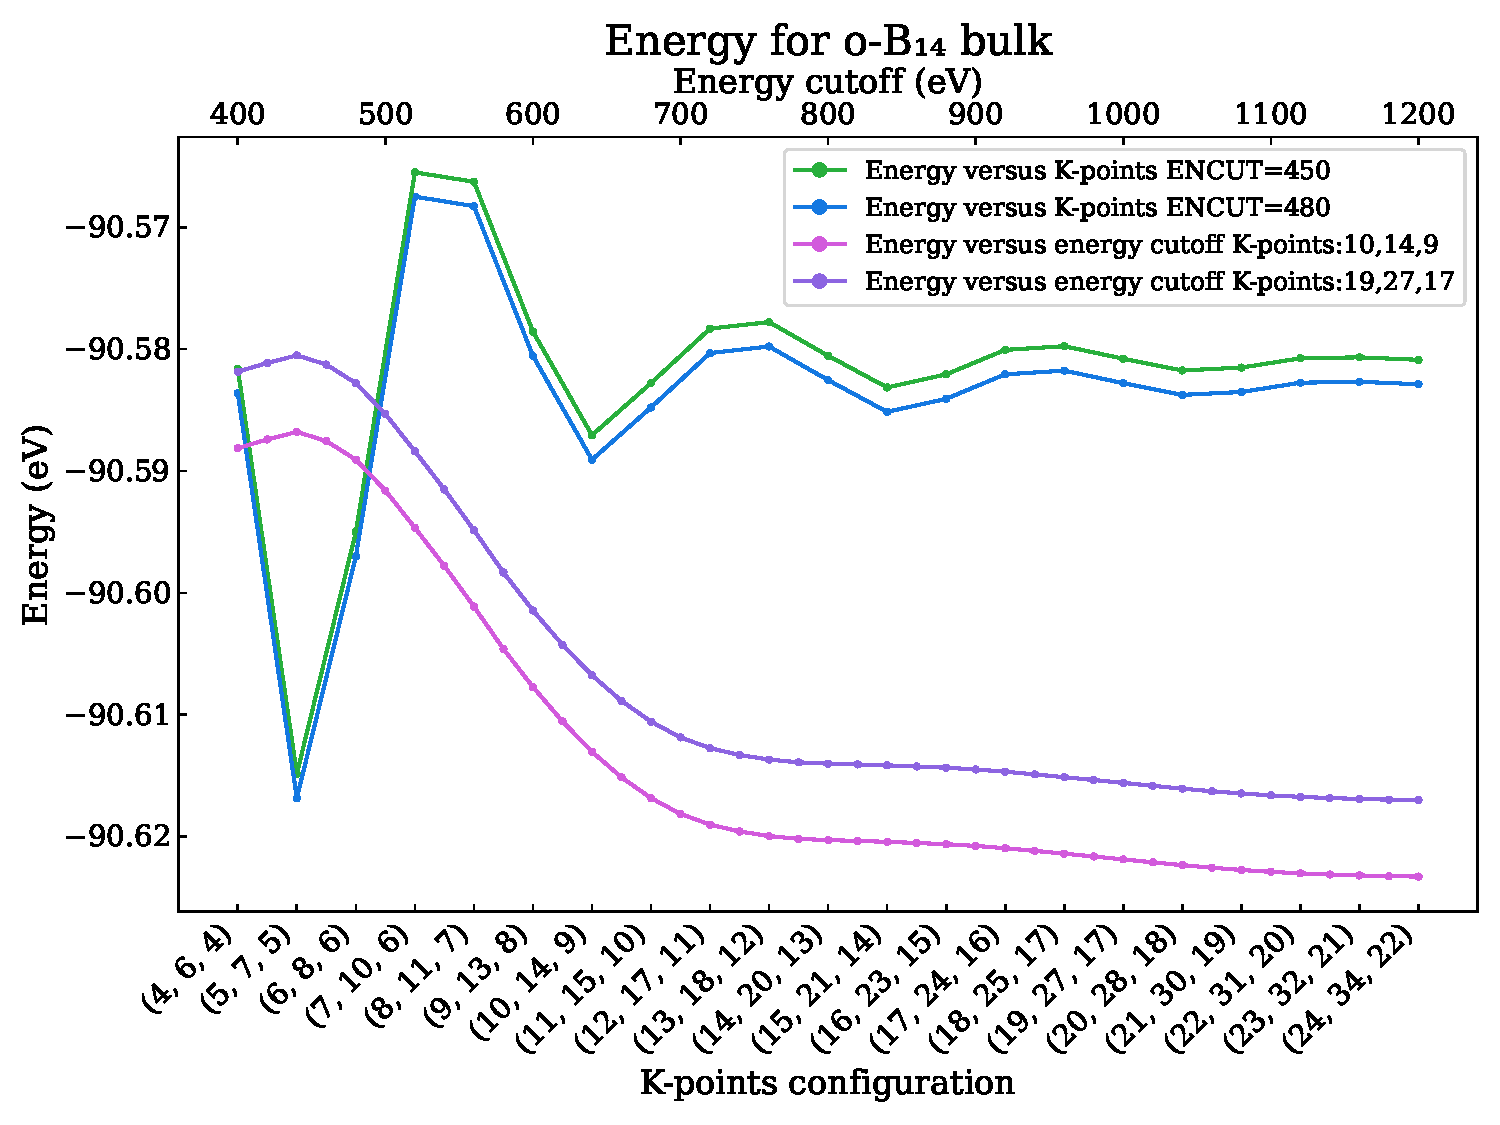
\includegraphics[width=0.6\linewidth]{figures_proj2/S2.1a.pdf}}%
    \par\nointerlineskip
    \adjustbox{valign=c}{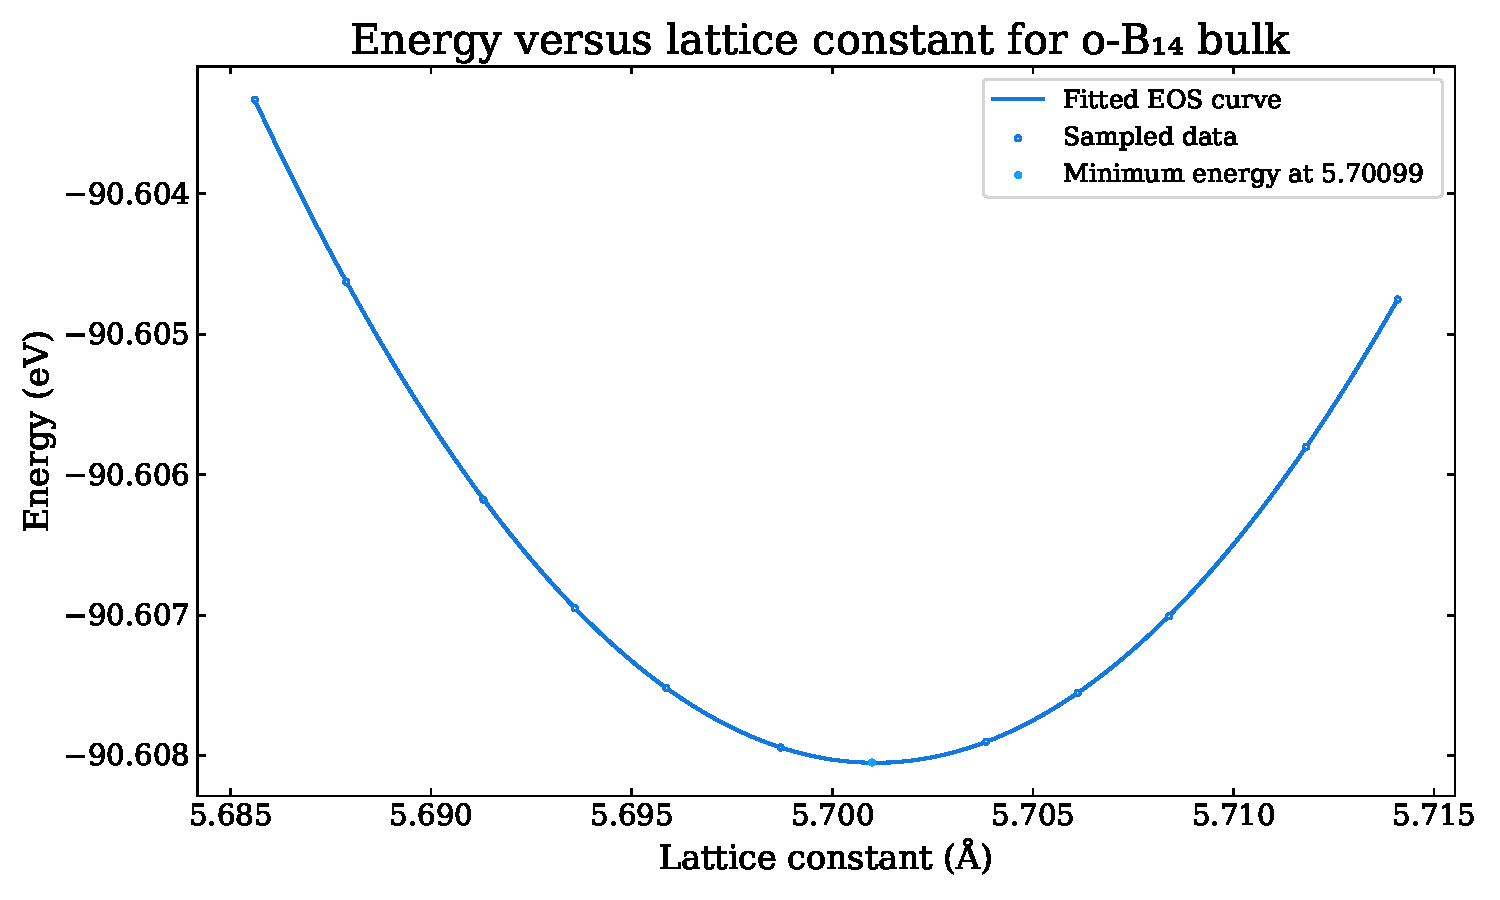
\includegraphics[width=0.6\linewidth]{figures_proj2/S2.1b.pdf}}%
\caption{Upper: Plane-wave energy cutoff and k-point convergence of the total energy for bulk o-\ce{B14};
Lower: Lattice-constant dependence of the total energy at a plane-wave energy cutoff of \qty{600}{\electronvolt} and a k-point set of $34\times48\times31$.}
\label{S2.1}
\end{figure}

\begin{figure}[!htbp]
\centering
    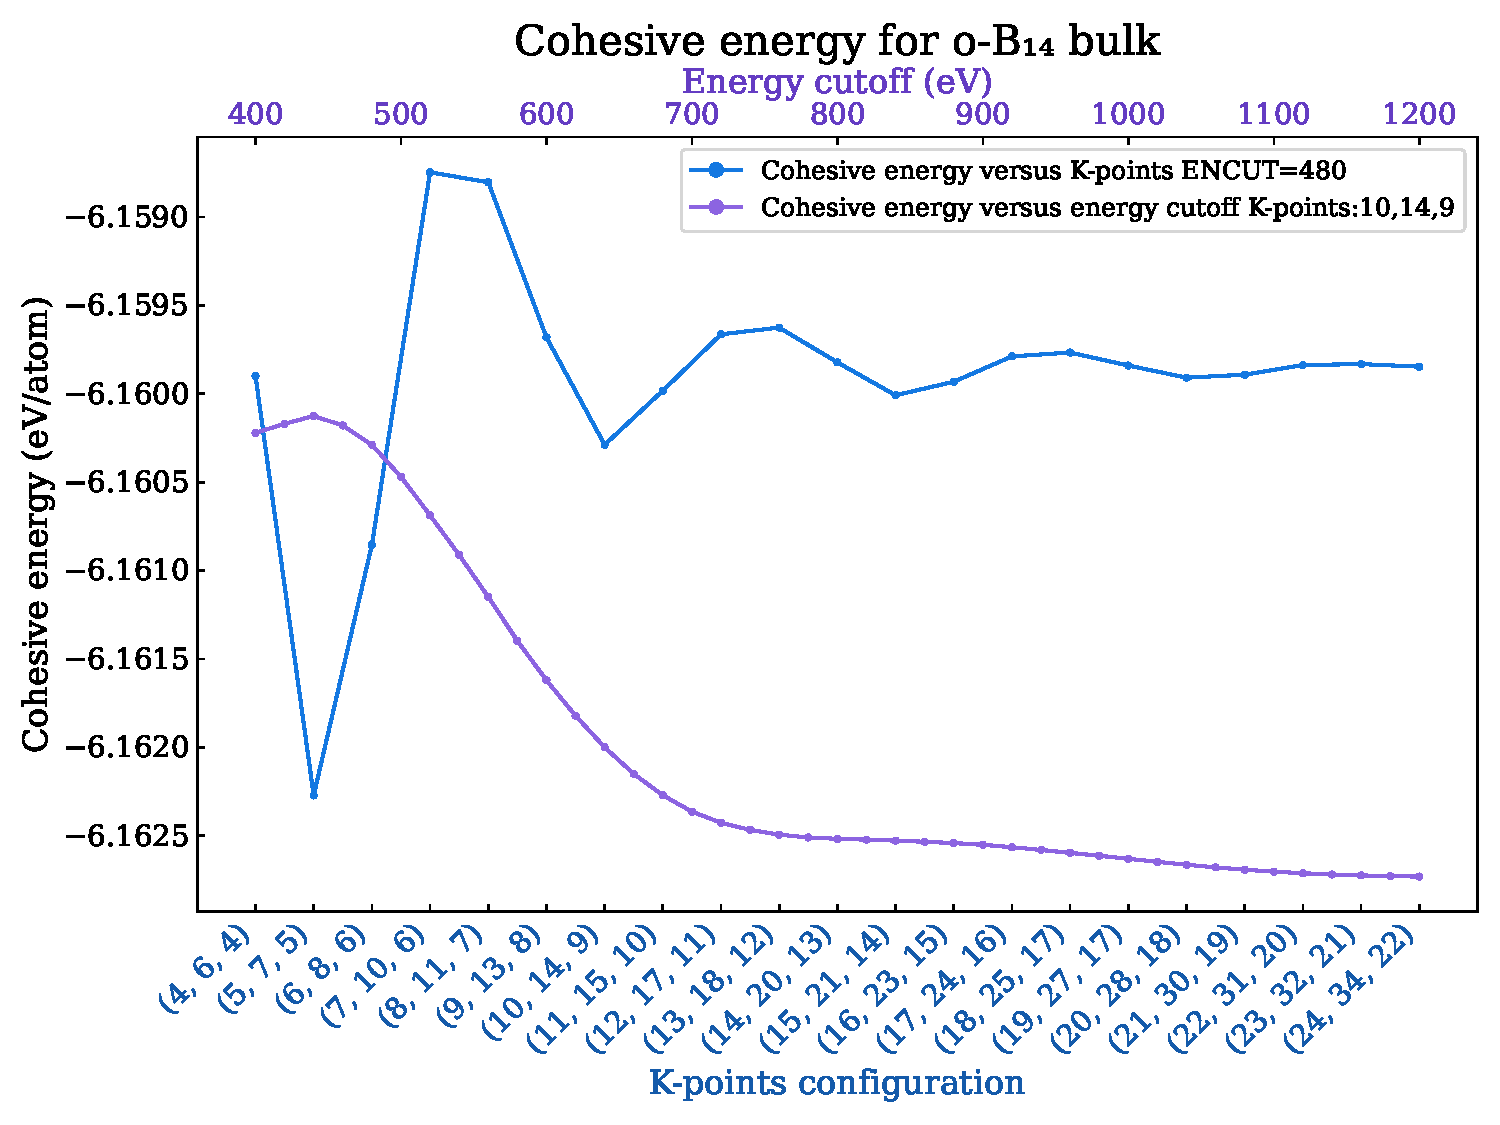
\includegraphics[width=0.6\linewidth]{figures_proj2/S2.2.pdf}
\caption{Cohesive energy per atom as a function of plane-wave energy cutoff and k-point set for bulk o-\ce{B14}.}
\label{S2.2}
\end{figure}

\begin{figure}[!htbp]
\centering
    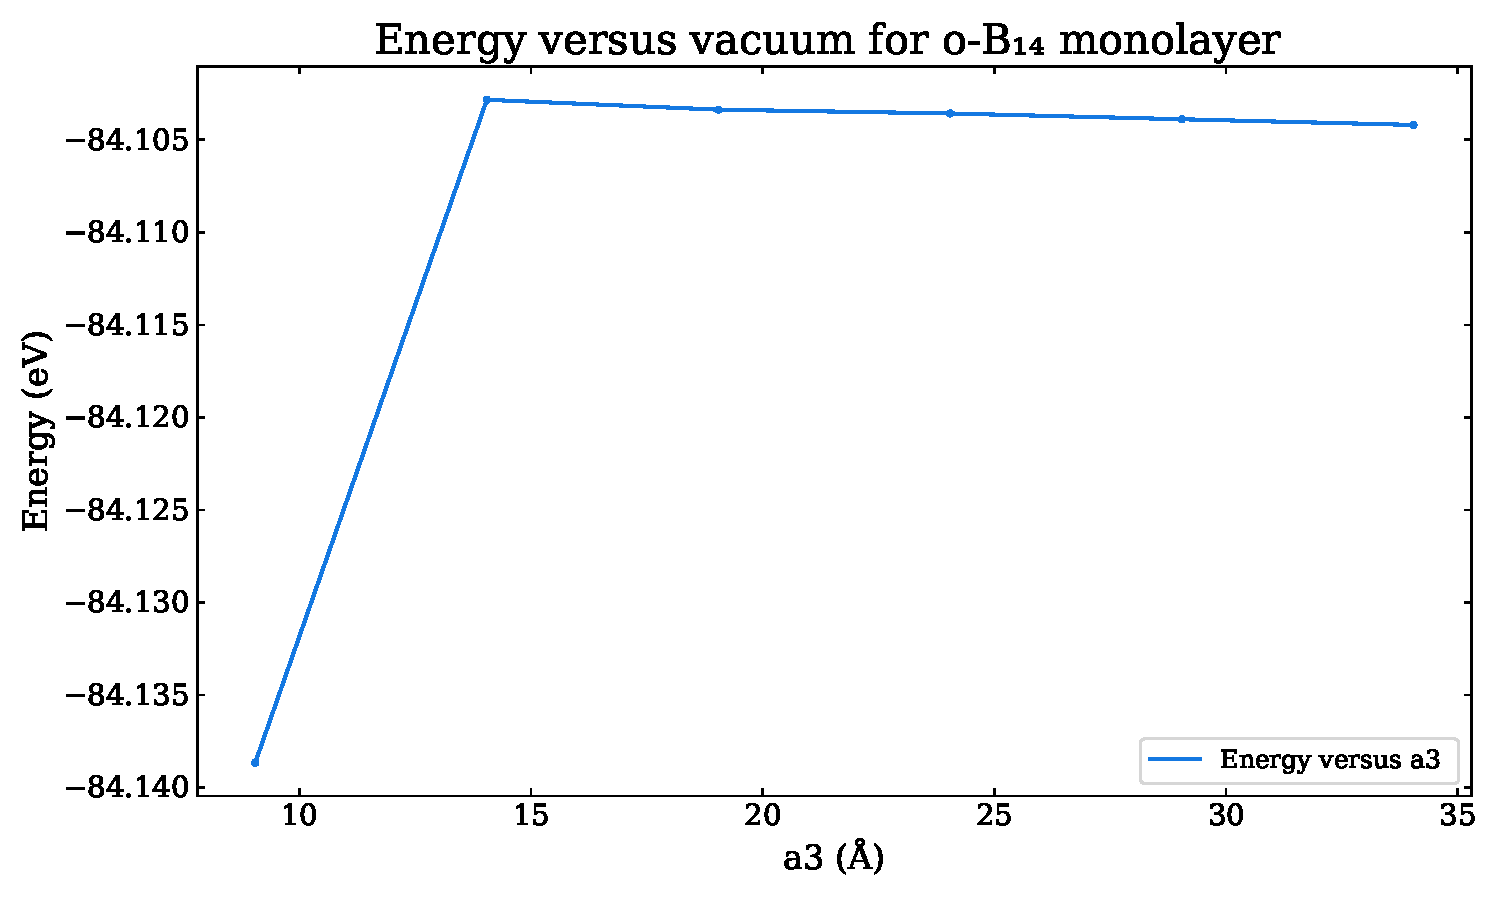
\includegraphics[width=0.6\linewidth]{figures_proj2/S2.3.pdf}
\caption{Total energy as a function of vacuum-region thickness.}
\label{S2.3}
\end{figure}

\begin{figure}[!htbp]
\centering
    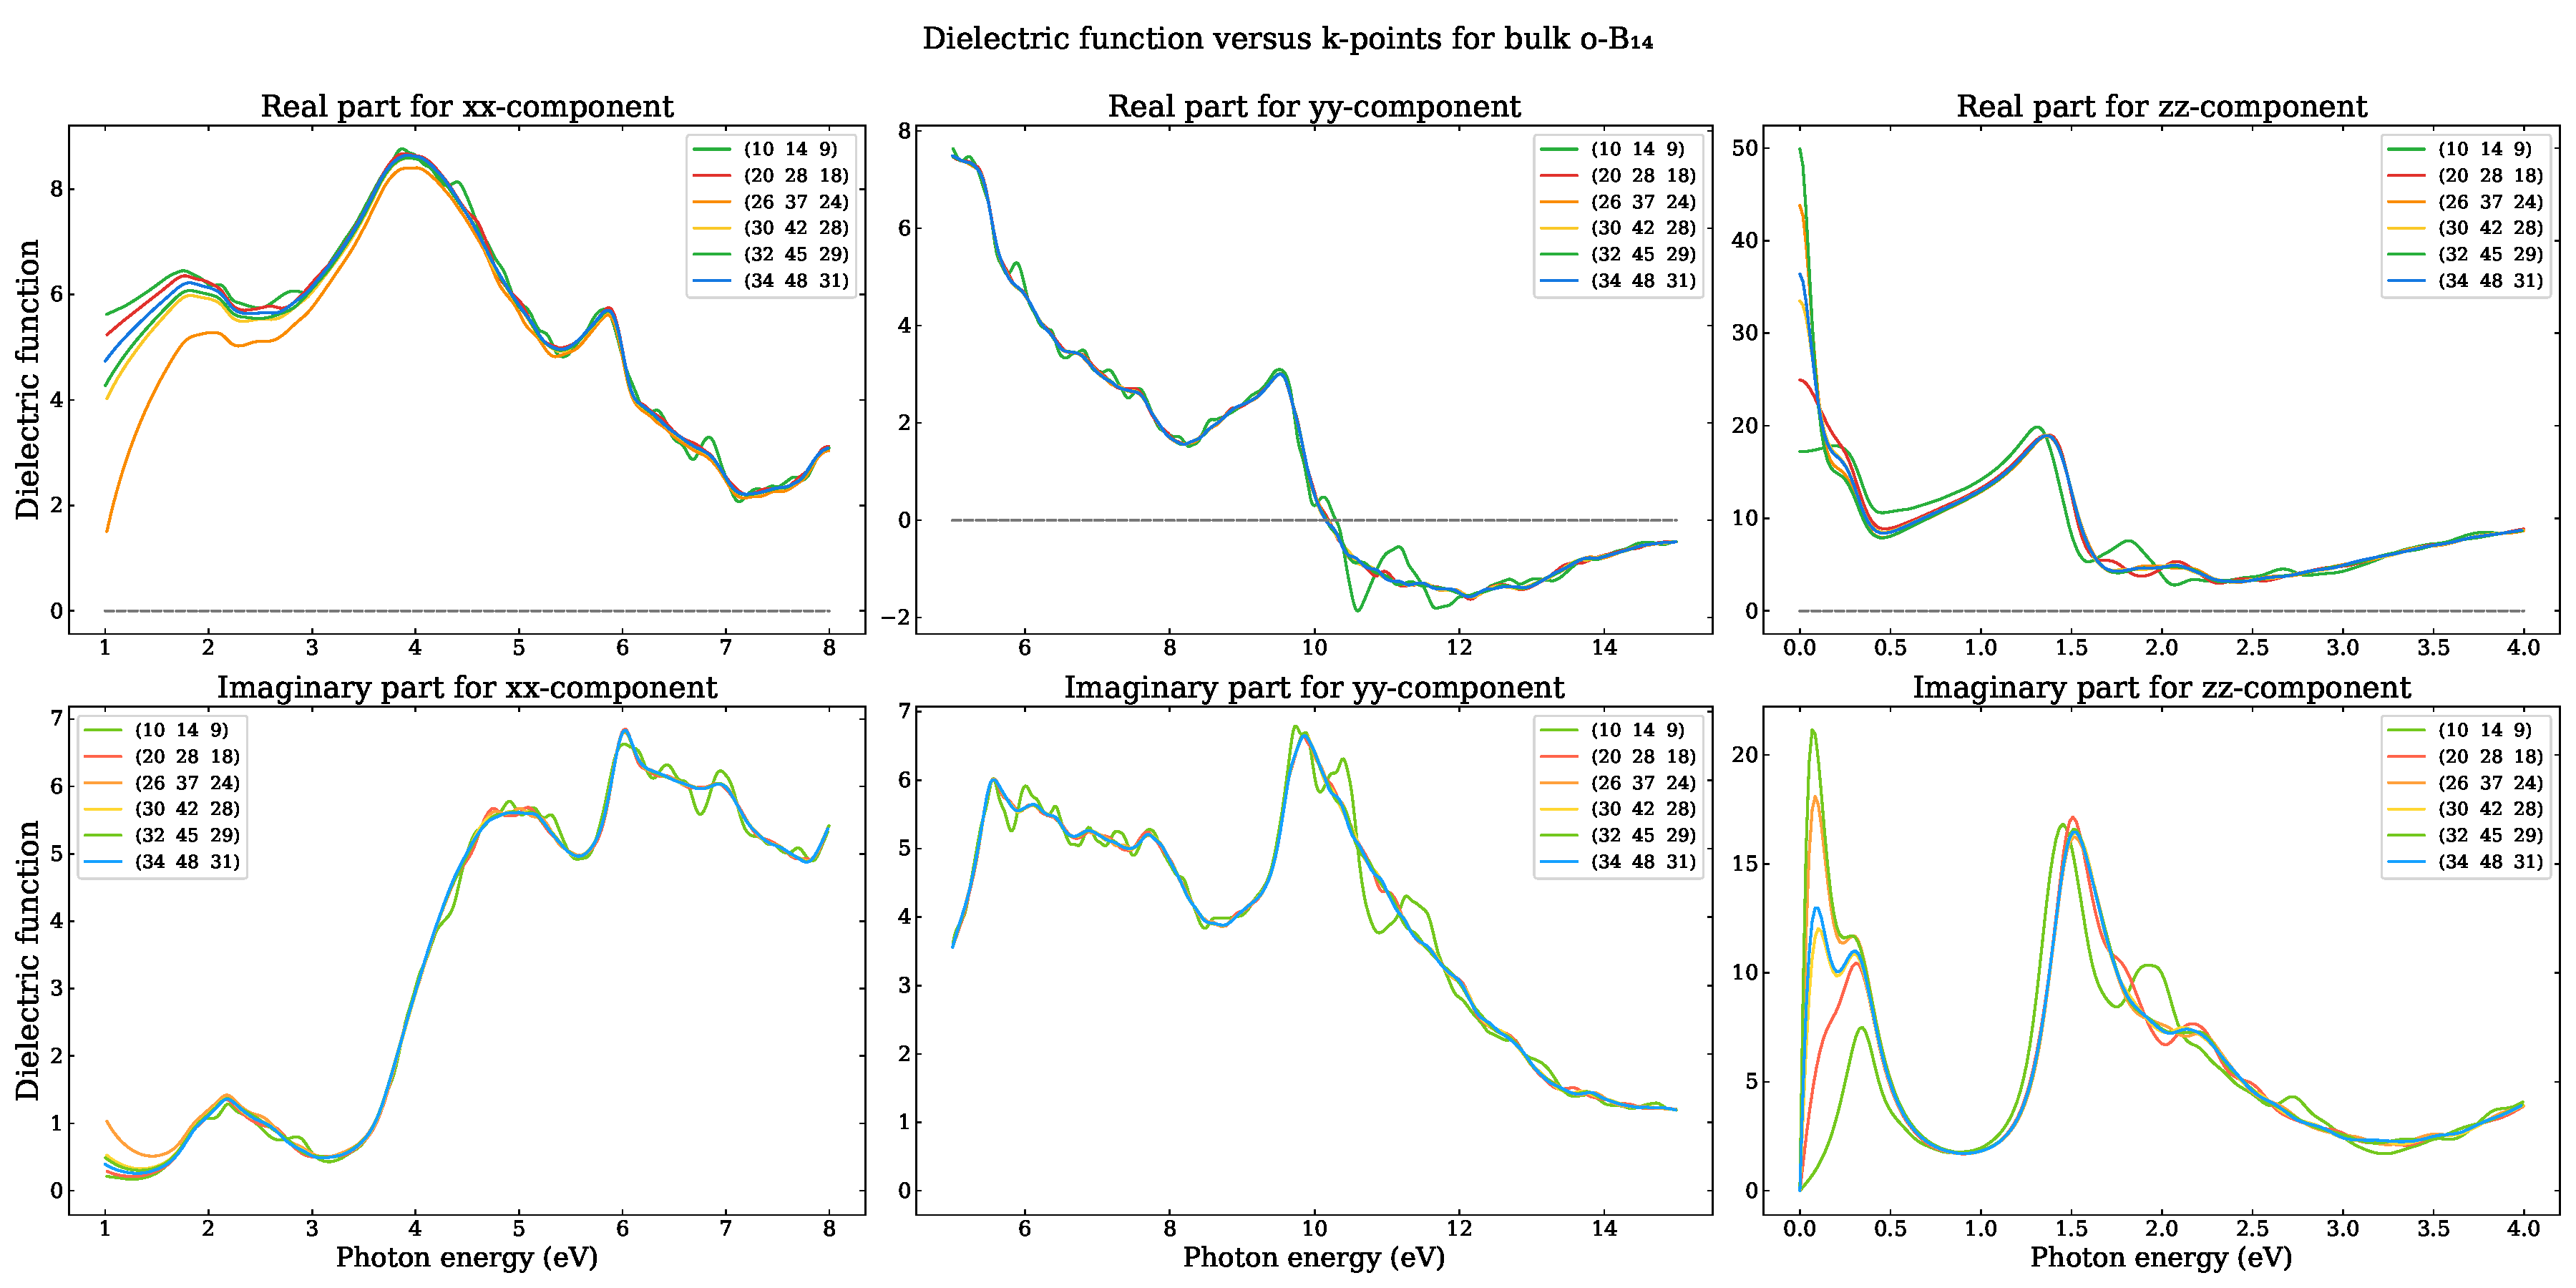
\includegraphics[width=1.0\linewidth]{figures_proj2/S2.4.pdf}
\caption{In-plane and out-of-plane components of the real and imaginary parts of the dielectric function of o-\ce{B14},
calculated with various k-point sets.}
\label{S2.4}
\end{figure}

\begin{figure}[!htbp]
\centering
    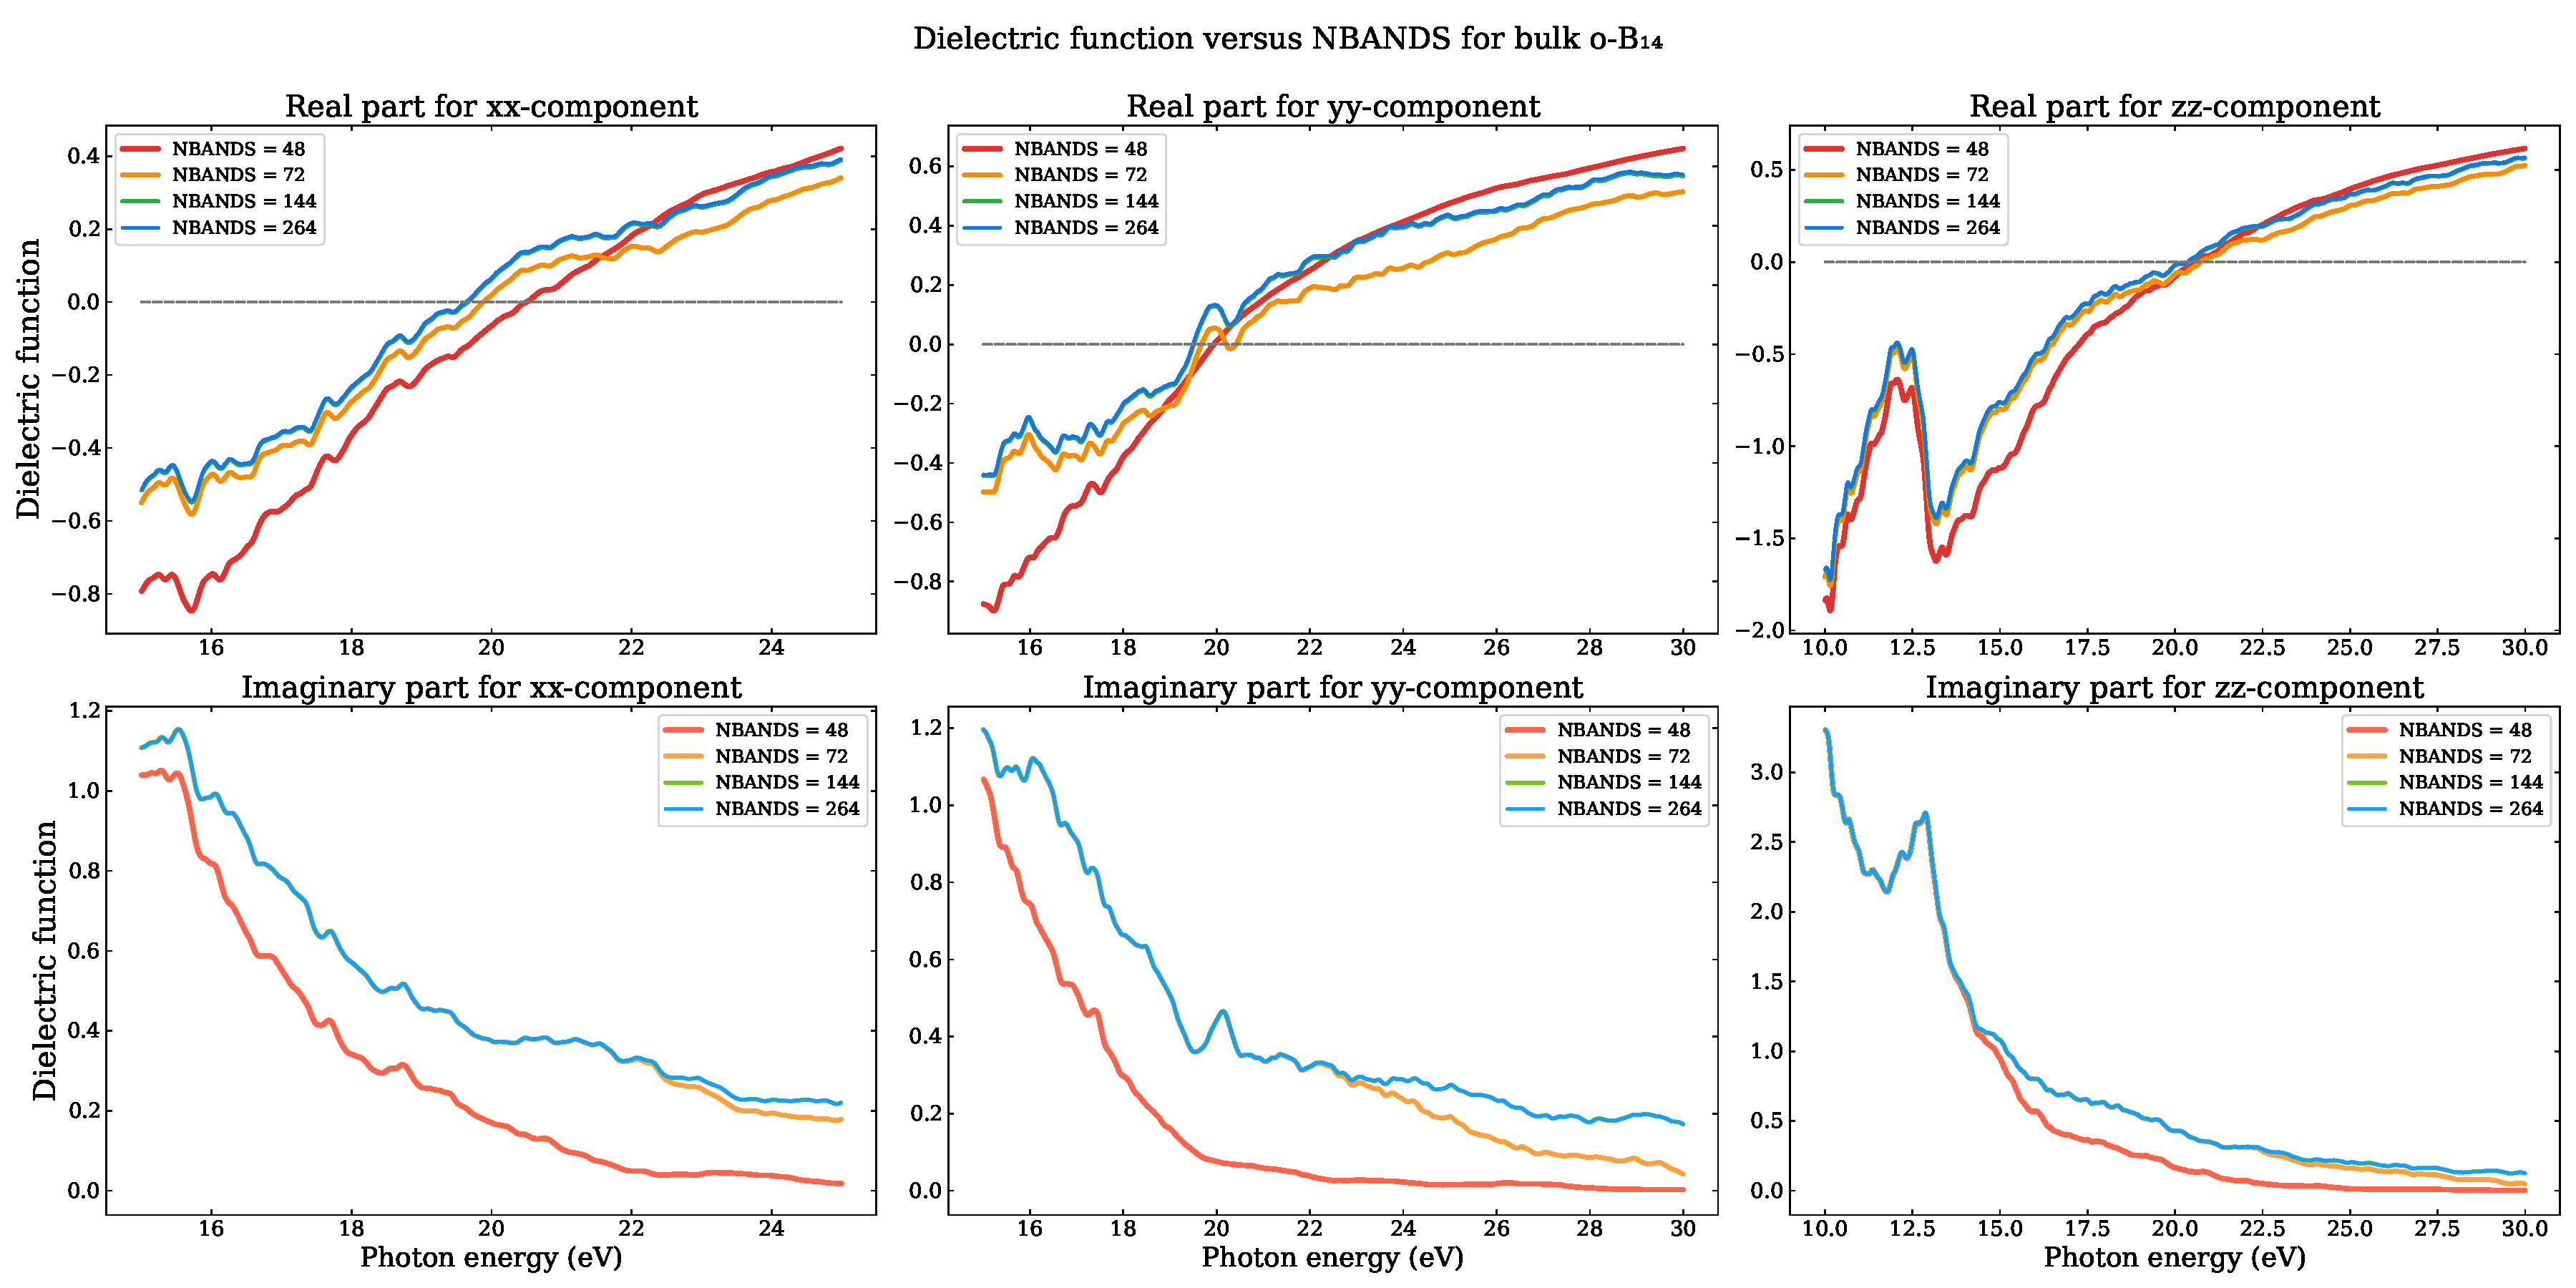
\includegraphics[width=1.0\linewidth]{figures_proj2/S2.5.pdf}
\caption{In-plane and out-of-plane components of the real and imaginary parts of the dielectric function of bulk o-\ce{B14},
calculated with different numbers of unoccupied states included in the calculation, as denoted by the parameter \texttt{NBANDS}.}
\label{S2.5}
\end{figure}

\begin{figure}[!htbp]
\centering
    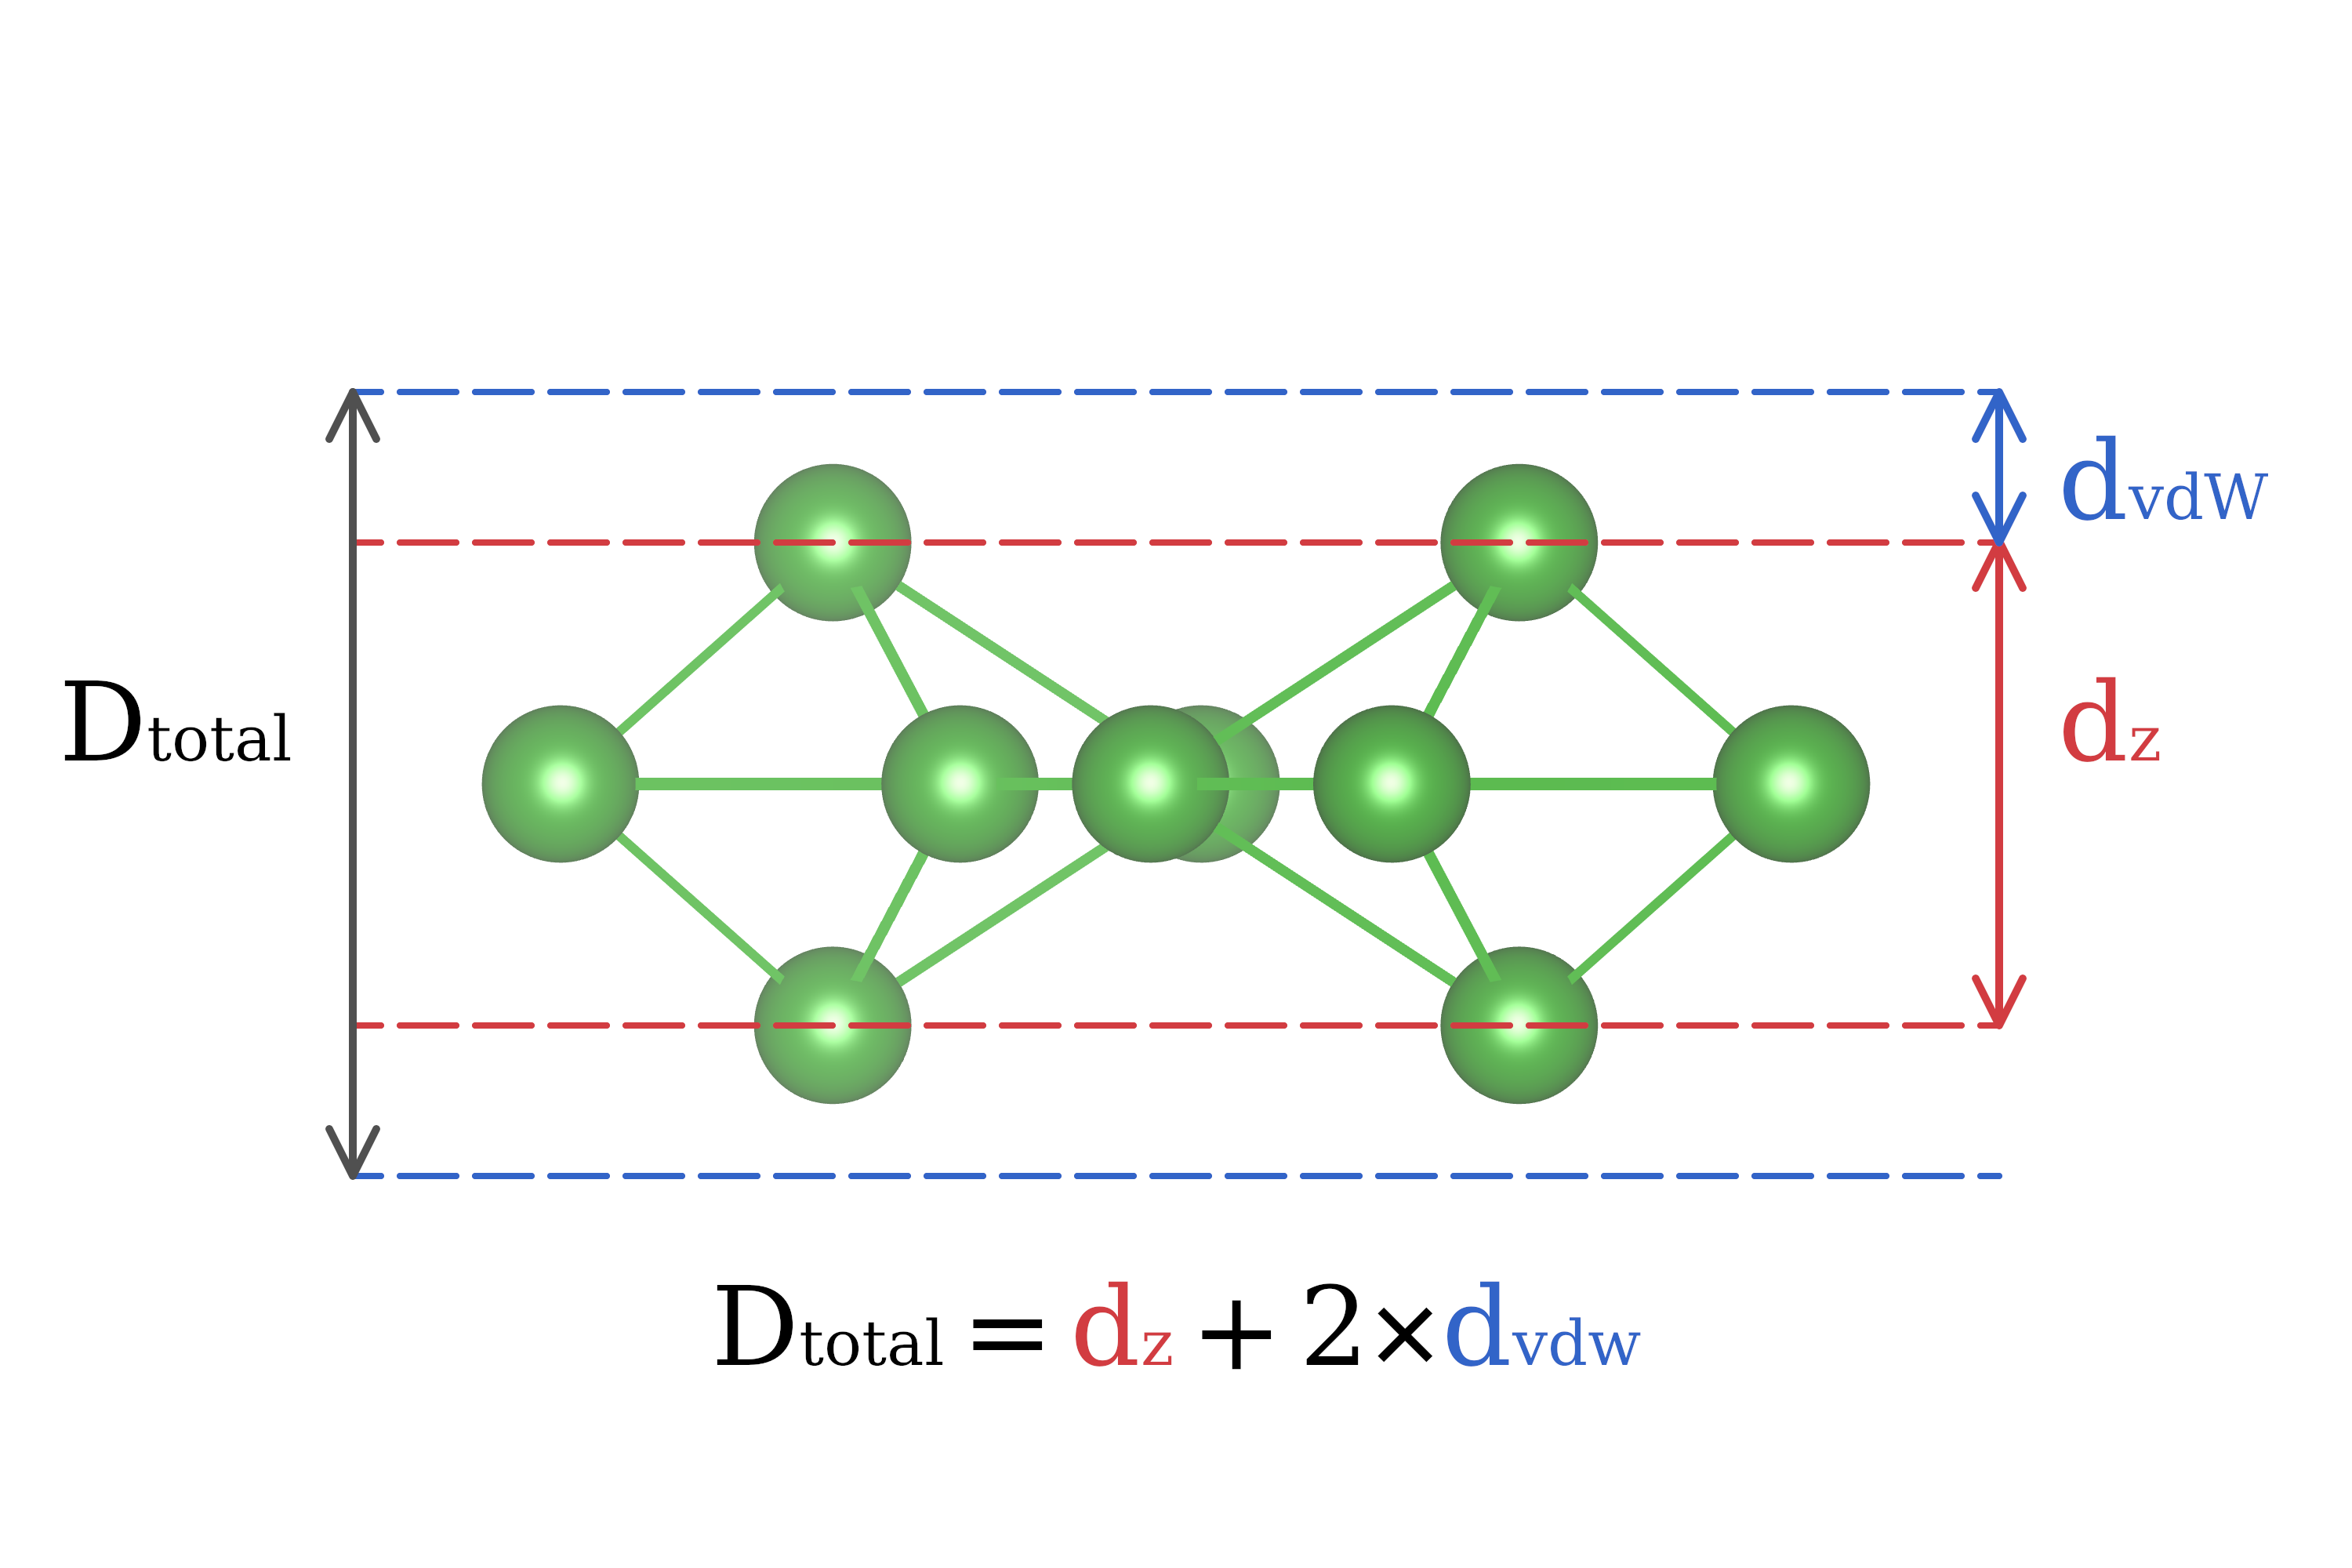
\includegraphics[width=0.6\linewidth]{figures_proj2/S2.6.png}
\caption{Definition of the layer thickness used in the renormalization of the dielectric function, $D_{\mathrm{total}} \coloneqq d_{\mathrm{2D}}$.}
\label{S2.6}
\end{figure}

\begin{figure}[!htbp]
\centering
    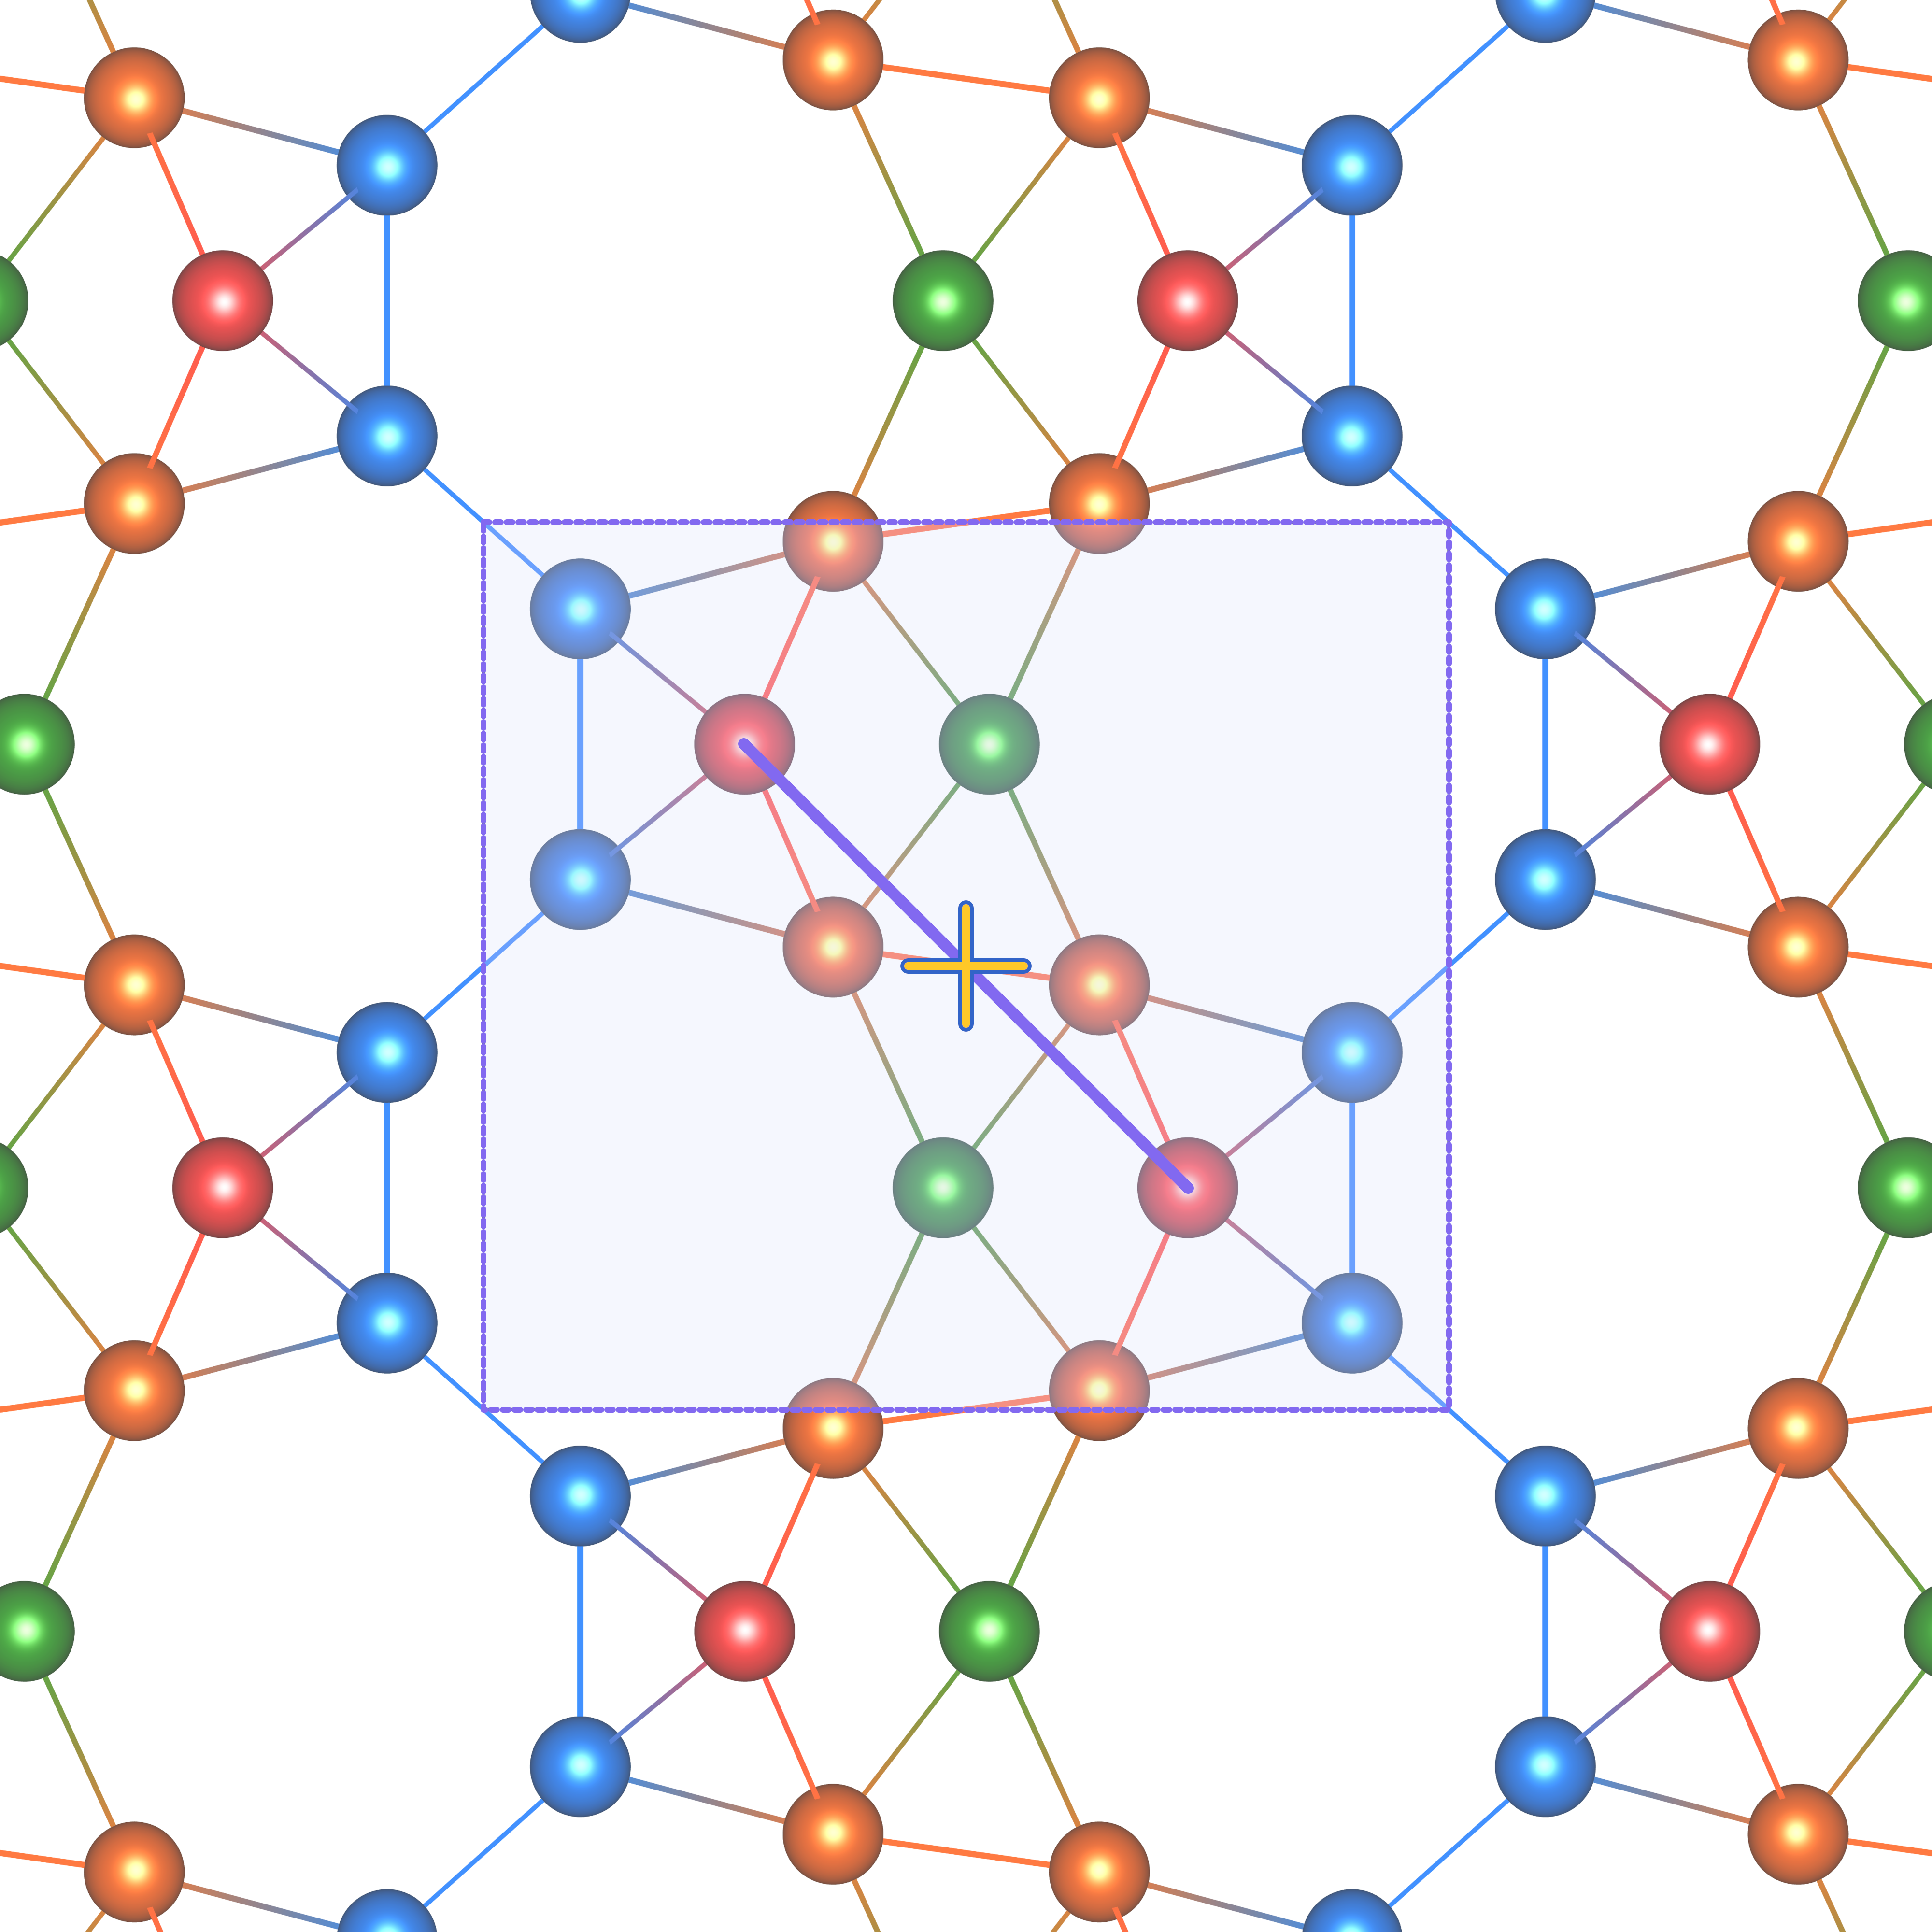
\includegraphics[width=0.6\linewidth]{figures_proj2/S2.7.png}
\caption{Sketch of the hollow-bridge site, indicated by the yellow cross,
for the hydrogen adsorption on the monolayer and bilayer structures.
The black rectangle represents the unit cell.}
\label{S2.7}
\end{figure}

\begin{figure}[!htbp]
\centering
    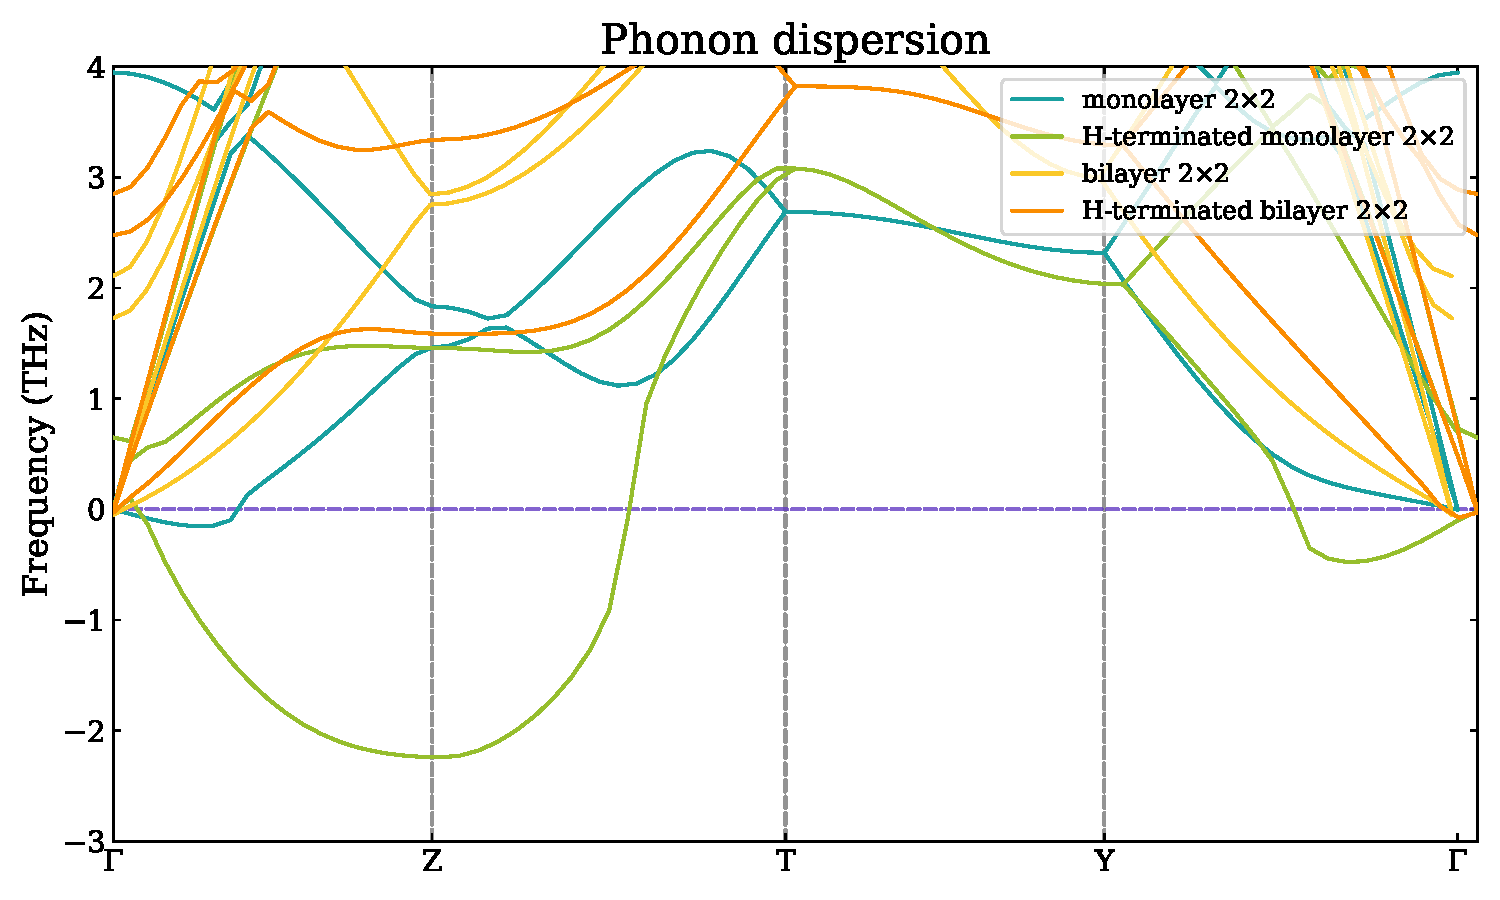
\includegraphics[width=0.6\linewidth]{figures_proj2/S2.8.pdf}
\caption{Phonon dispersion curves obtained using a $(2\times2)$ supercell.}
\label{S2.8}
\end{figure}

\begin{figure}[!htbp]
\centering
    \adjustbox{valign=c}{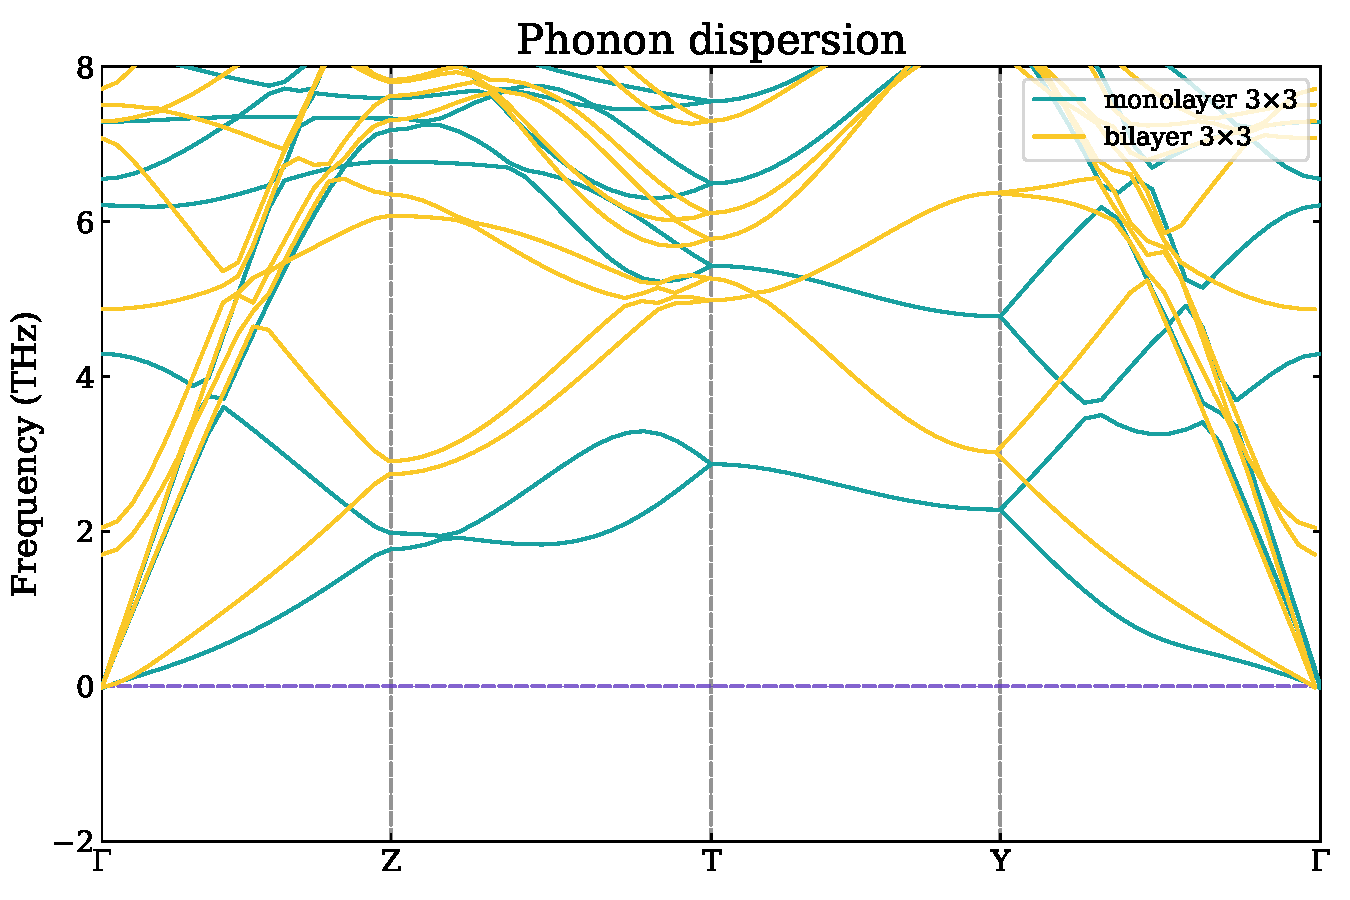
\includegraphics[width=0.45\linewidth]{figures_proj2/S2.9a.pdf}}%
    \adjustbox{valign=c}{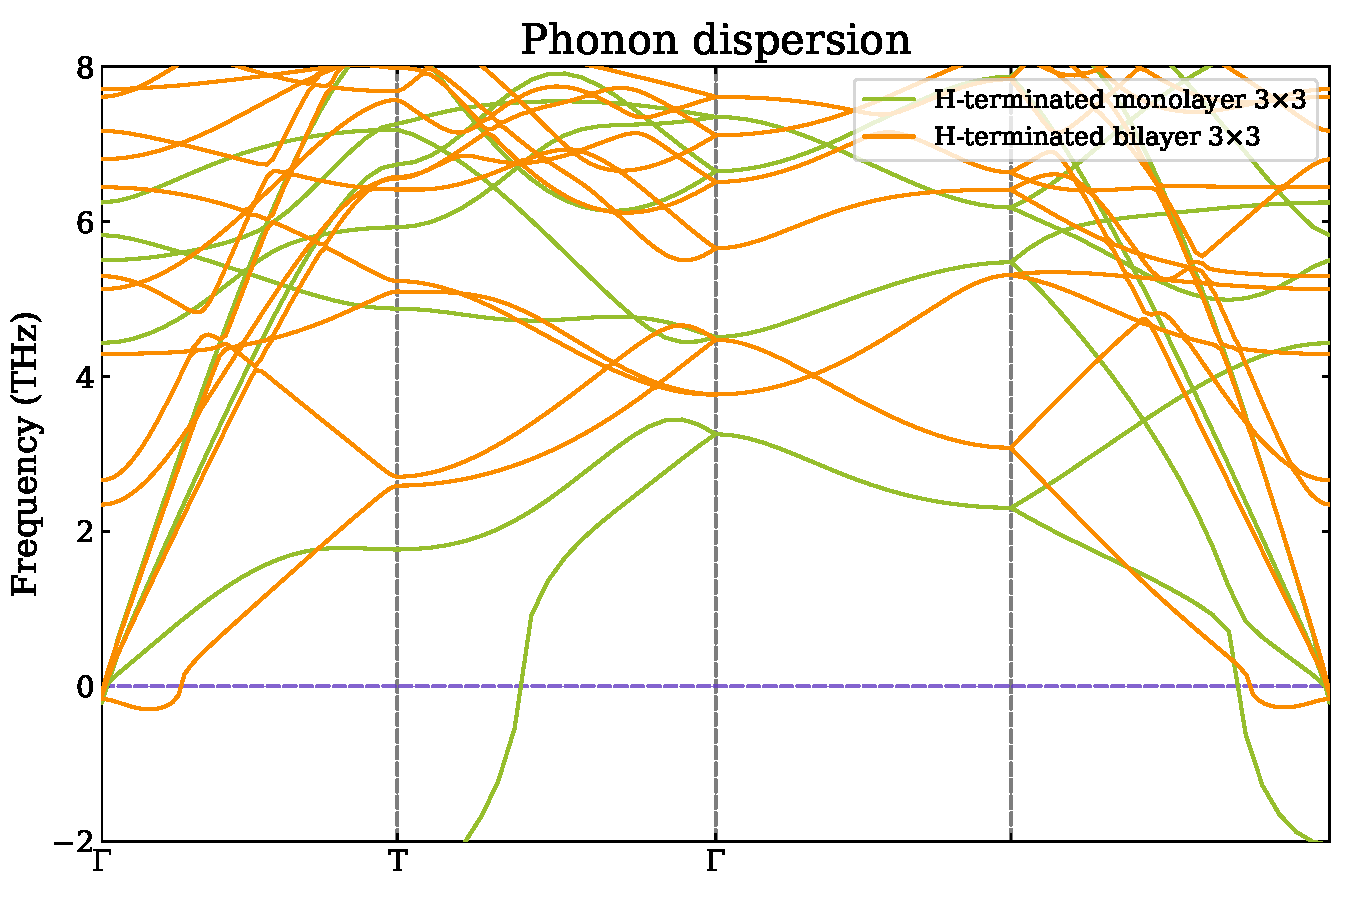
\includegraphics[width=0.45\linewidth]{figures_proj2/S2.9b.pdf}}%
\caption{Left: Phonon dispersion curves of the monolayer and bilayer calculated using a $3\times3$ supercell;
Right: Phonon dispersion curves of the hydrogen-terminated monolayer and bilayer calculated using a $3\times3$ supercell.
Small negative frequencies appear around the $\Gamma$ point for the hydrogen-terminated bilayer.
These small negative frequencies are often found in 2D materials and do not by themselves indicate dynamical instability~\cite{liu2016continuum,querne2023crystal,pallikara2022physical}.}
\label{S2.9}
\end{figure}

\begin{figure}[!htbp]
\centering
    \adjustbox{valign=c}{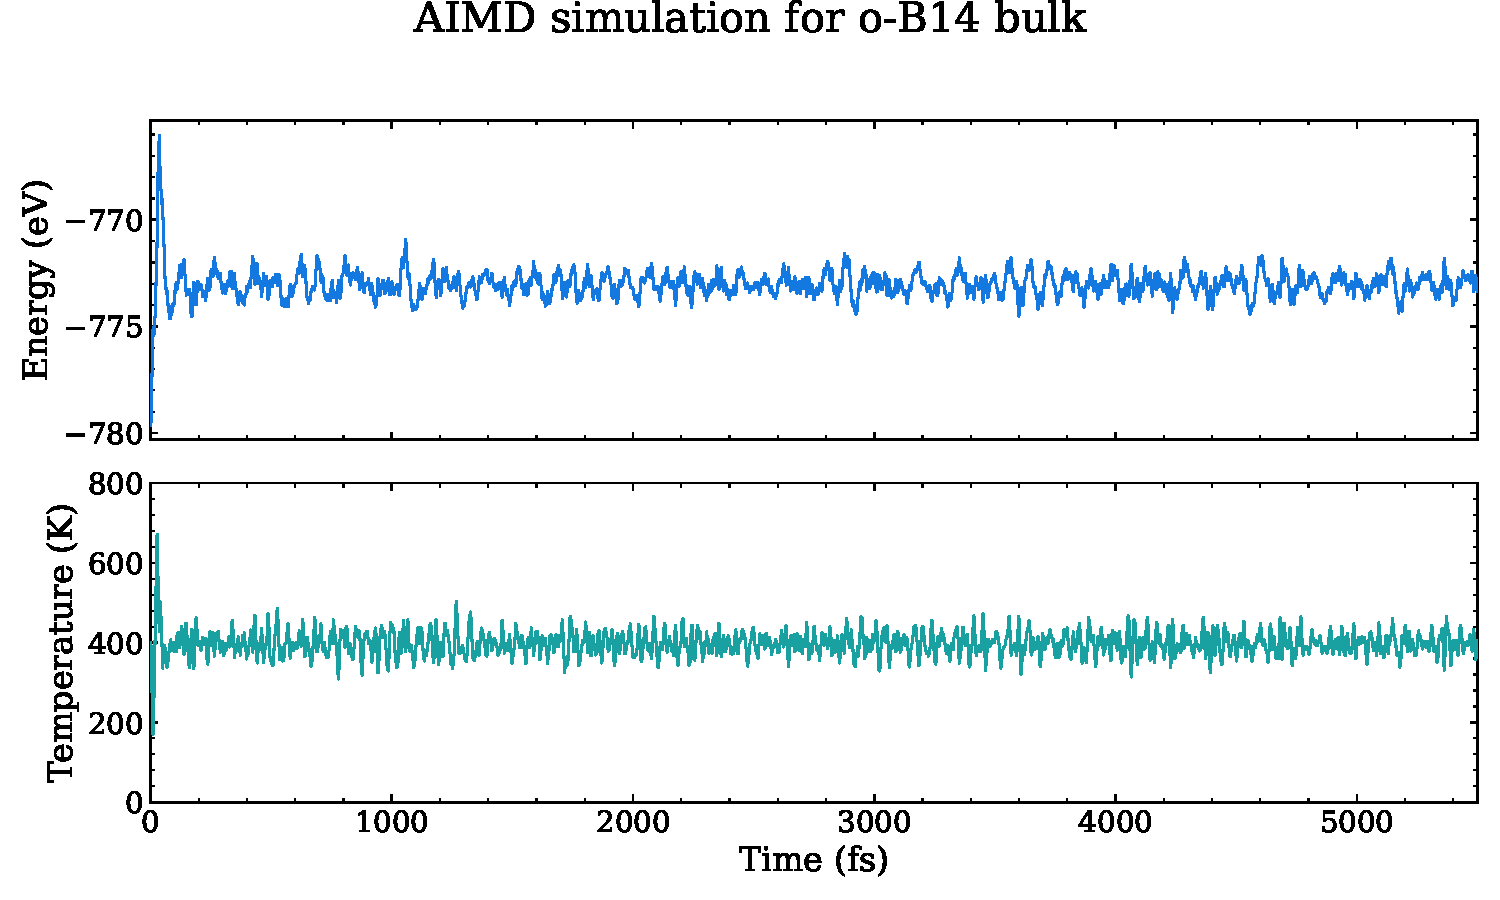
\includegraphics[width=0.75\linewidth]{figures_proj2/S2.10/S2.10a_long.pdf}}%
    \adjustbox{valign=c}{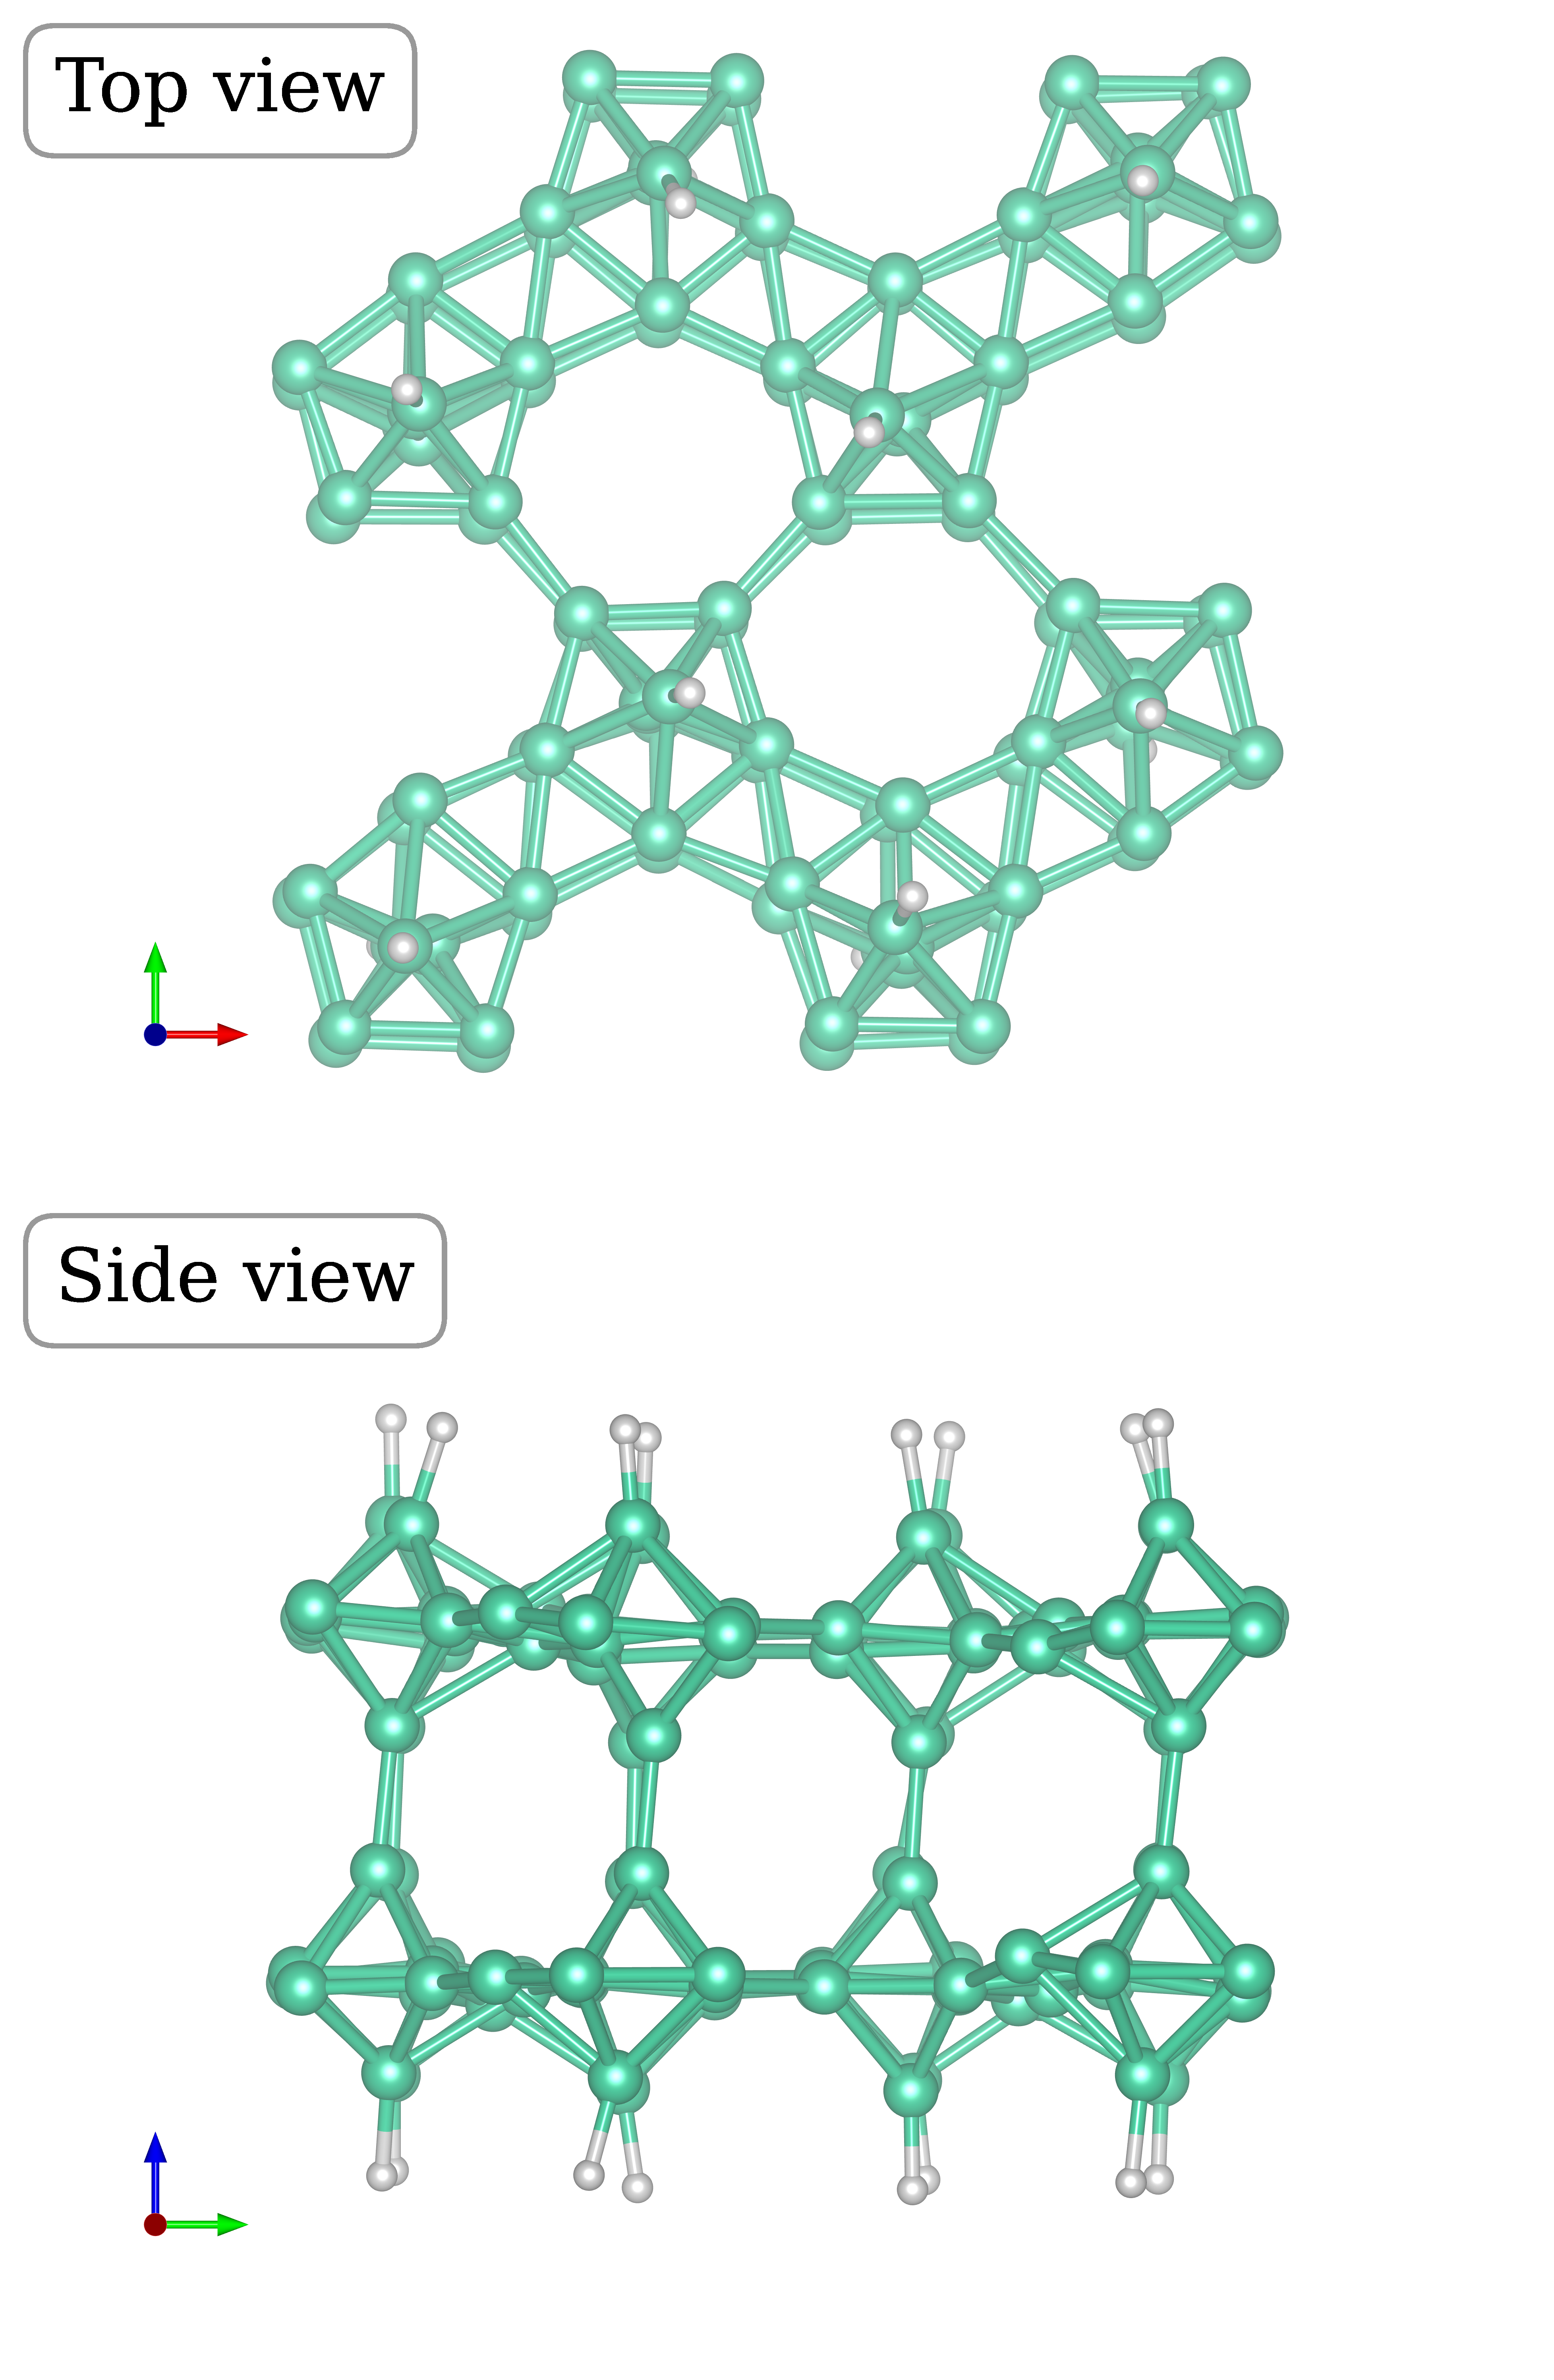
\includegraphics[width=0.25\linewidth]{figures_proj2/S2.10/S2.10b.pdf}}%
\caption{
Left: Total energy and temperature as functions of time from \textit{ab initio} molecular dynamics calculations for the hydrogen-terminated bilayer at \qty{400}{K};
Right: Top and side views of the molecular structure of the hydrogen-terminated bilayer at the corresponding temperature.
The structure remains structurally stable and exhibits only minimal deformation.}
\label{S2.10}
\end{figure}

\begin{figure}[!htbp]
\centering
    \adjustbox{valign=c}{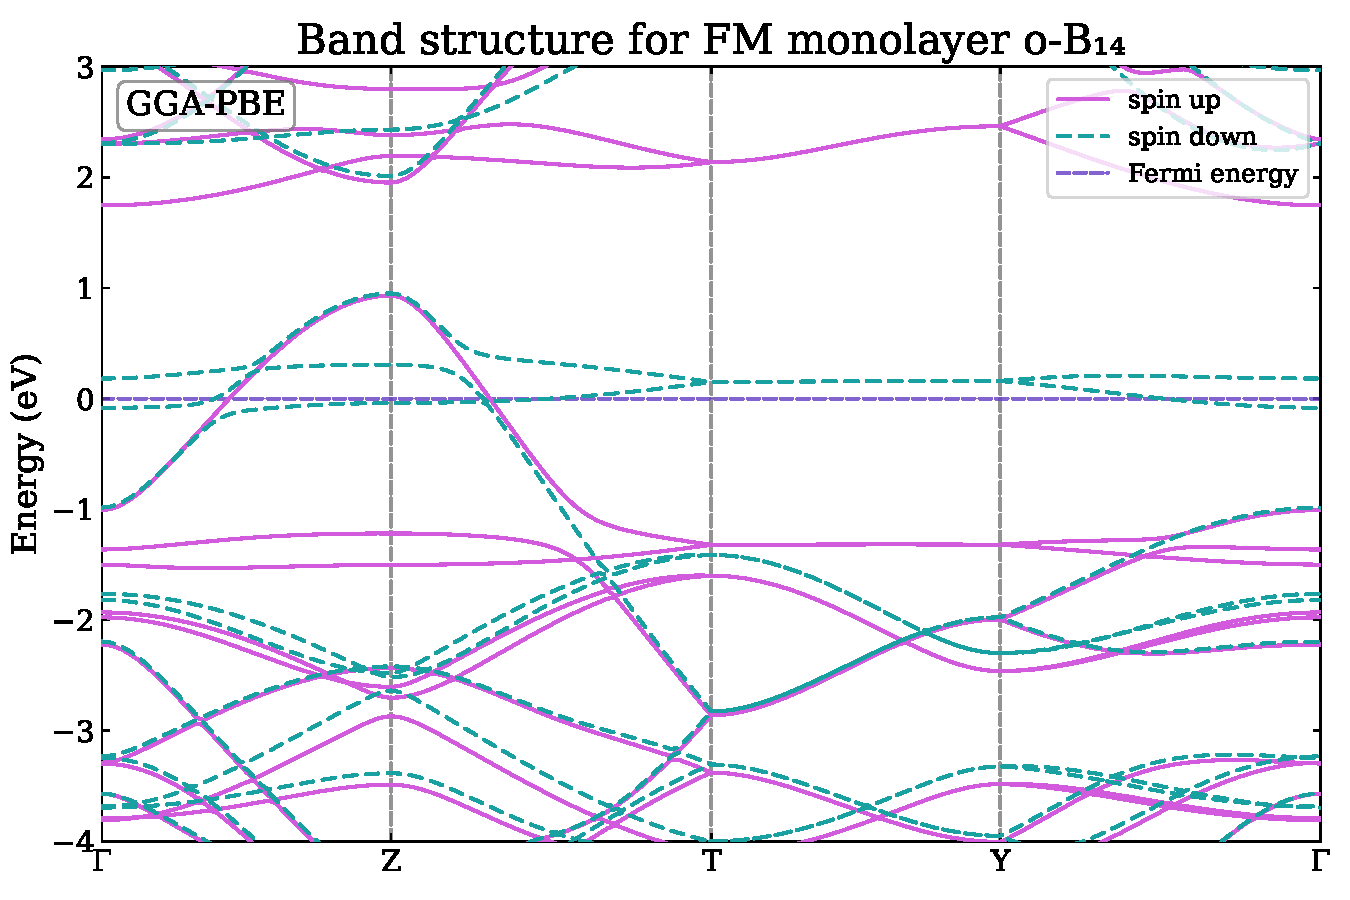
\includegraphics[width=0.45\linewidth]{figures_proj2/S2.11a.pdf}}%
    \adjustbox{valign=c}{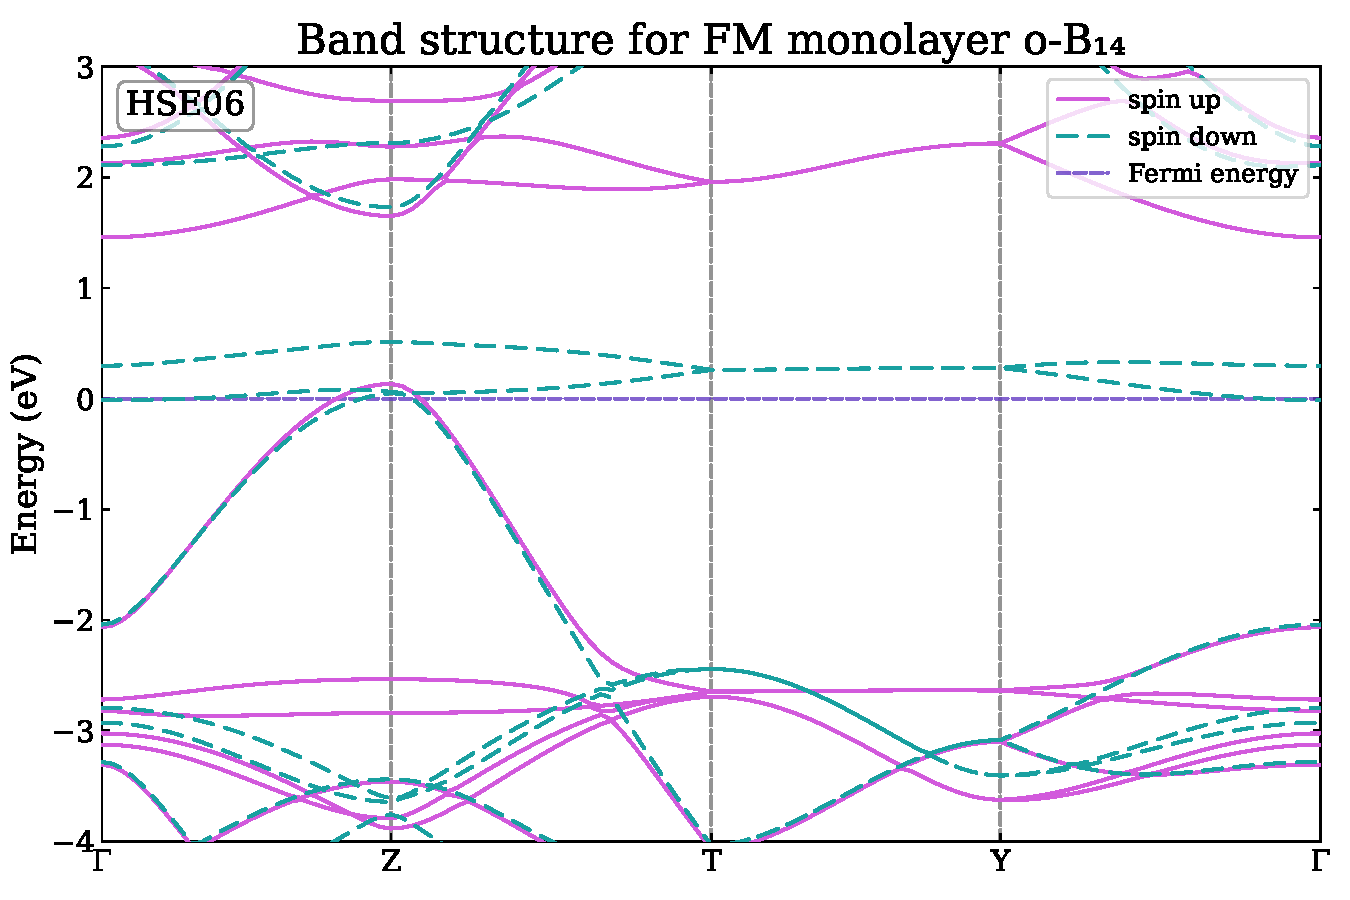
\includegraphics[width=0.45\linewidth]{figures_proj2/S2.11b.pdf}}%
\caption{
Left: Spin-polarized ferromagnetic band structure of the monolayer calculated using the PBE functional;
Right: Spin-polarized ferromagnetic band structure of the monolayer calculated using the HSE06 functional.}
\label{S2.11}
\end{figure}

\begin{figure}[!htbp]
\centering
    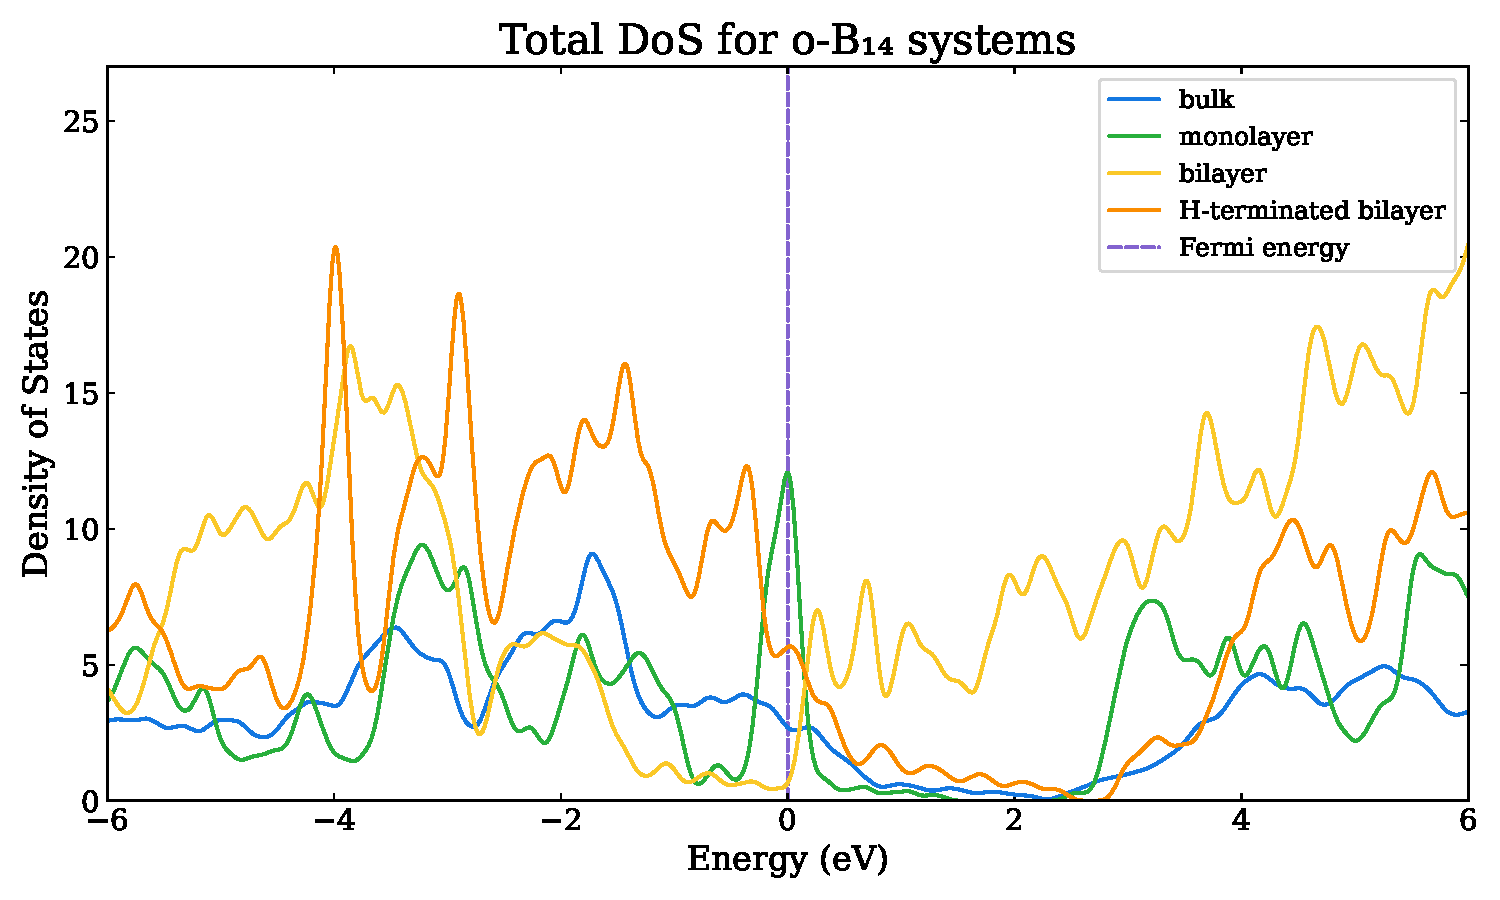
\includegraphics[width=0.6\linewidth]{figures_proj2/S2.12.pdf}
\caption{Total density of states (DoS) of the various structures as calculated using the PBE functional.}
\label{S2.12}
\end{figure}

\begin{figure}[!htbp]
\centering
    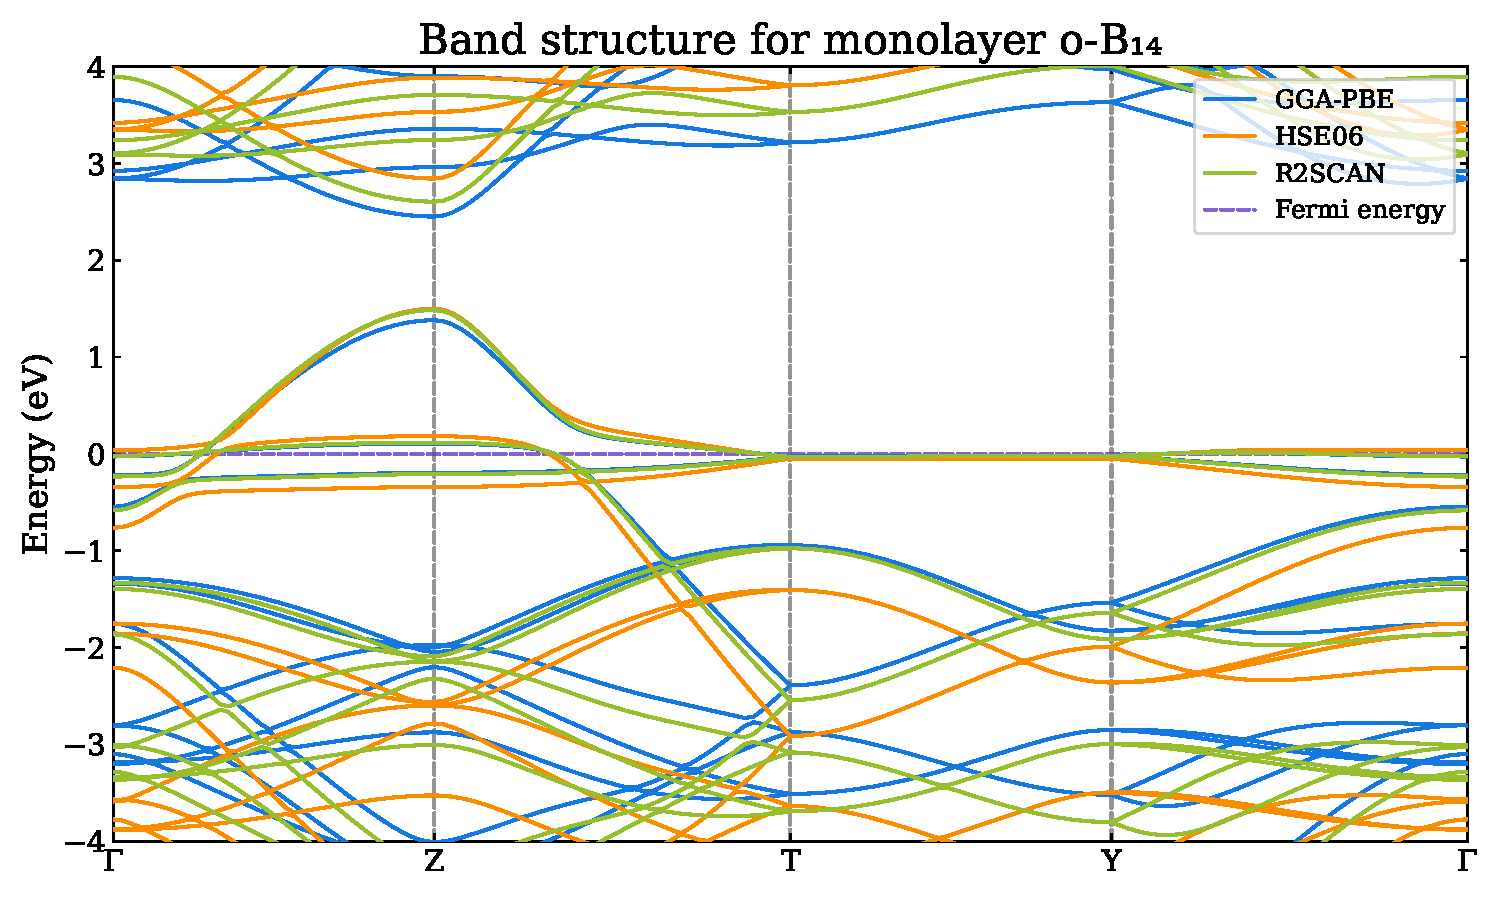
\includegraphics[width=0.6\linewidth]{figures_proj2/S2.13.pdf}
\caption{Non-spin-polarized band structure of the monolayer calculated using different functionals.}
\label{S2.13}
\end{figure}

\begin{figure}[!htbp]
\centering
    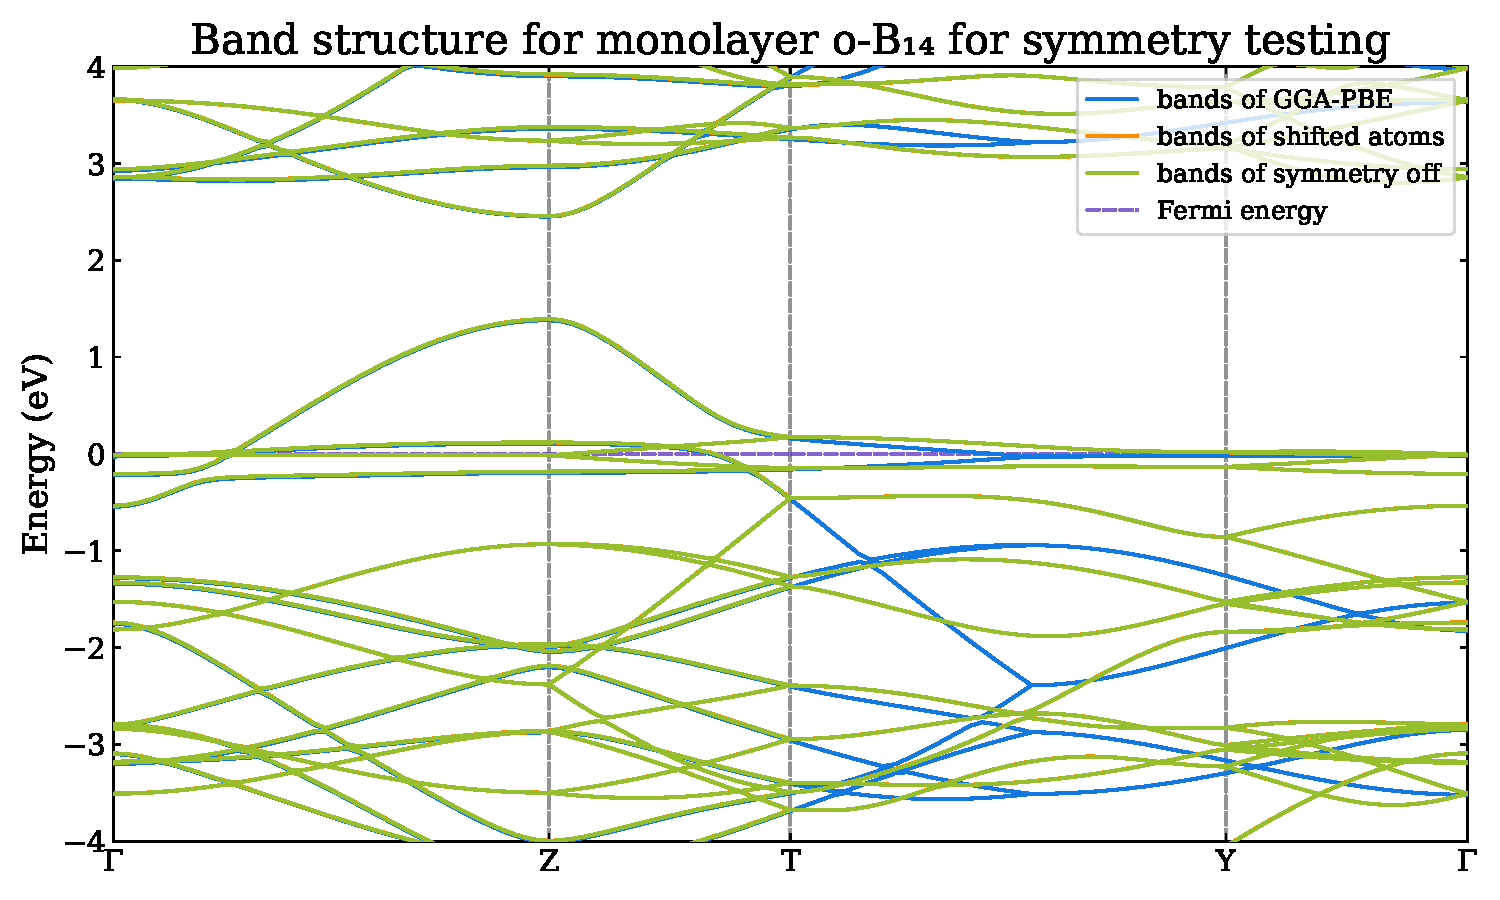
\includegraphics[width=0.6\linewidth]{figures_proj2/S2.14.pdf}
\caption{
Band structure of the monolayer calculated using a $(2\times1)$ unit cell.
The label ``shifted atoms'' means that,
in the initial atomic structure,
some atoms were moved slightly away from the ideal high-symmetry sites to break symmetry and allow Jahn--Teller distortions if they were favourable.
The structure was subsequently fully relaxed,
but the results remained unchanged and displayed no symmetry-lowering distortions.}
\label{S2.14}
\end{figure}

\begin{figure}[!htbp]
\centering
    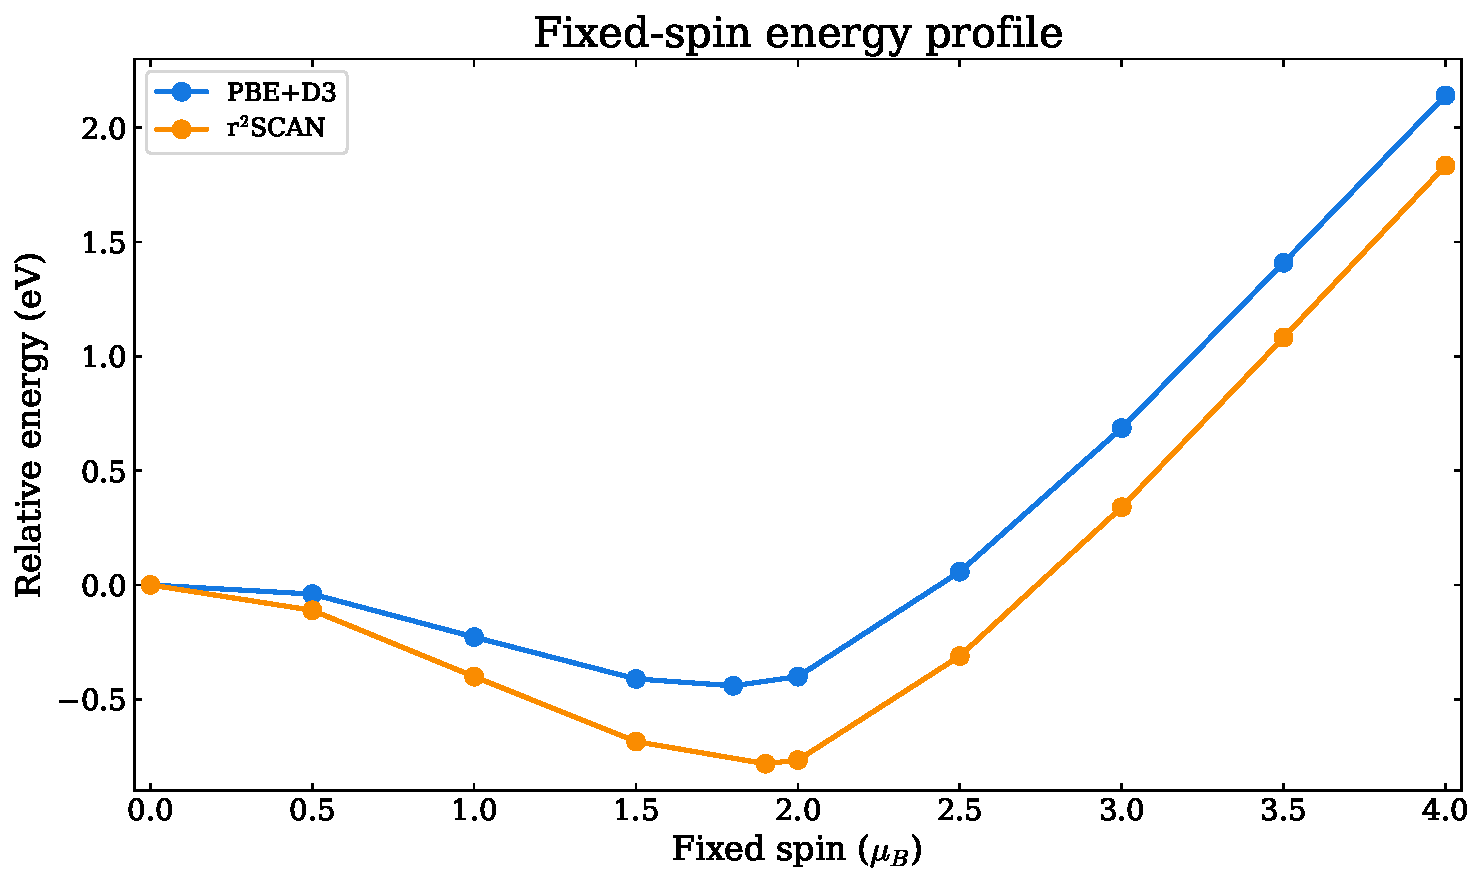
\includegraphics[width=0.6\linewidth]{figures_proj2/S2.15/S2.15.pdf}
\caption{Fixed-spin energy profile of the monolayer calculated using the PBE+D3 and r$^{2}$SCAN functionals.
The relative energy reaches its minimum near a fixed spin moment of $2.0~\mu_{\mathrm{B}}$.}
\label{S2.15}
\end{figure}

\begin{figure}[!htbp]
\centering
    \adjustbox{valign=c}{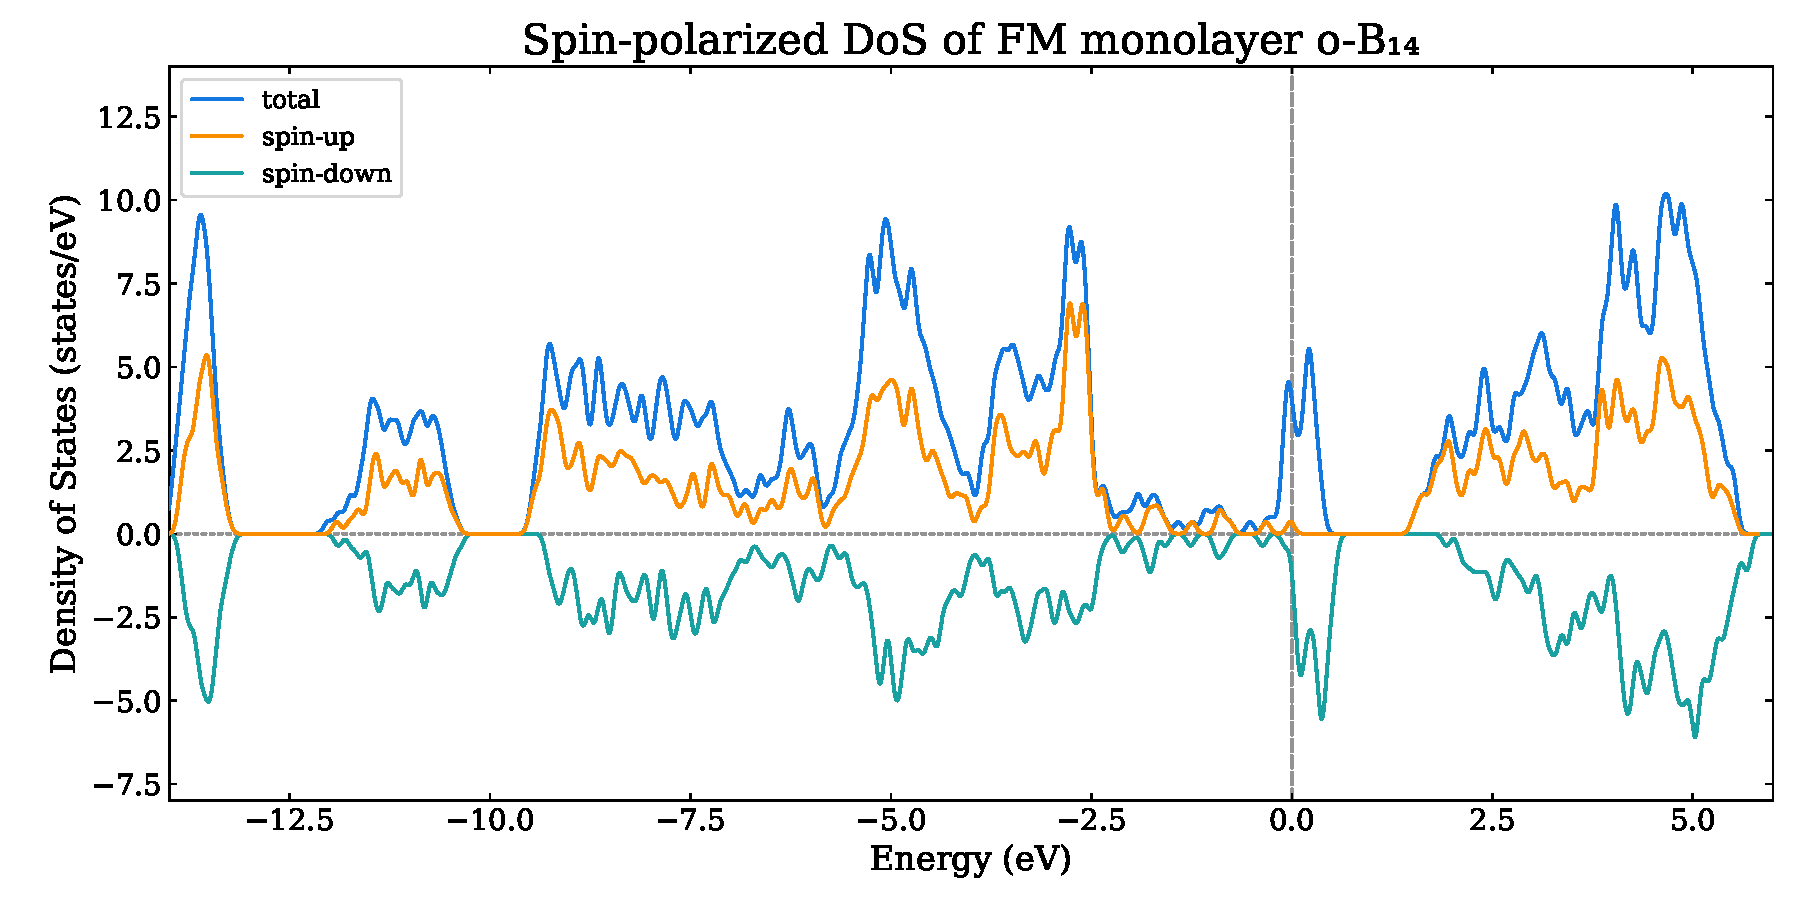
\includegraphics[width=0.6\linewidth]{figures_proj2/S2.16a.pdf}}%
    \par\nointerlineskip
    \adjustbox{valign=c}{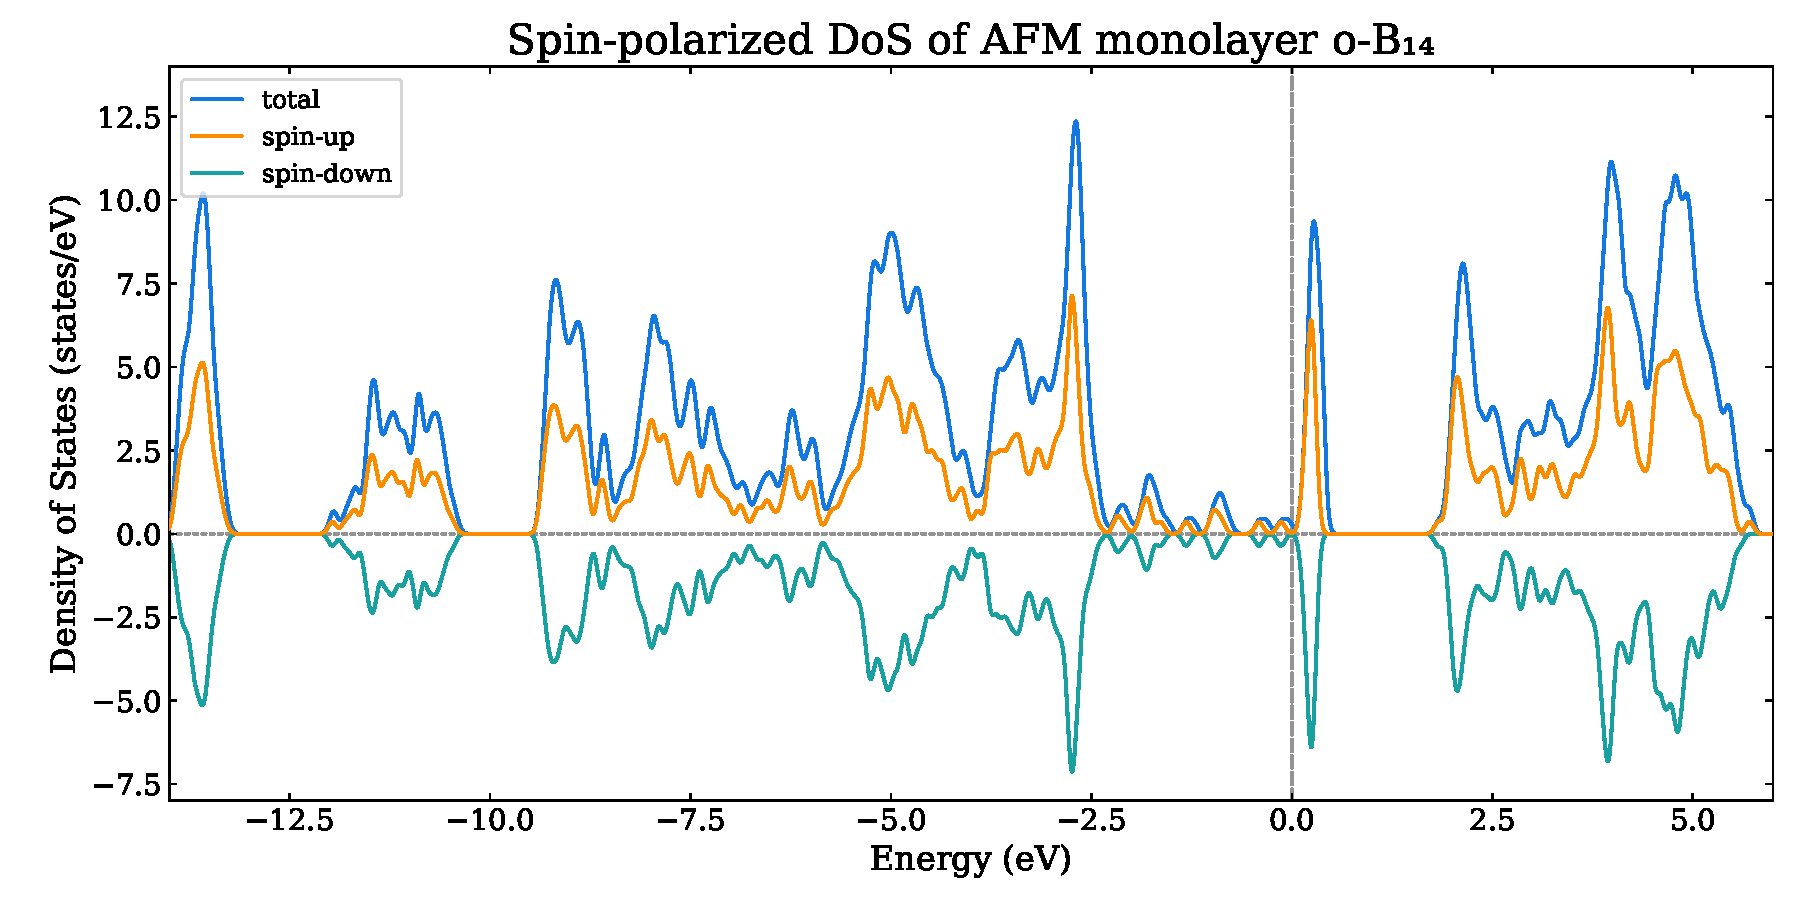
\includegraphics[width=0.6\linewidth]{figures_proj2/S2.16b.pdf}}%
\caption{Upper: Spin-resolved total DoS for the FM monolayer structure;
Lower: spin-resolved total DoS for the AFM monolayer structure,
as calculated using the HSE06 functional.}
\label{S2.16}
\end{figure}

\begin{figure}[!htbp]
\centering
    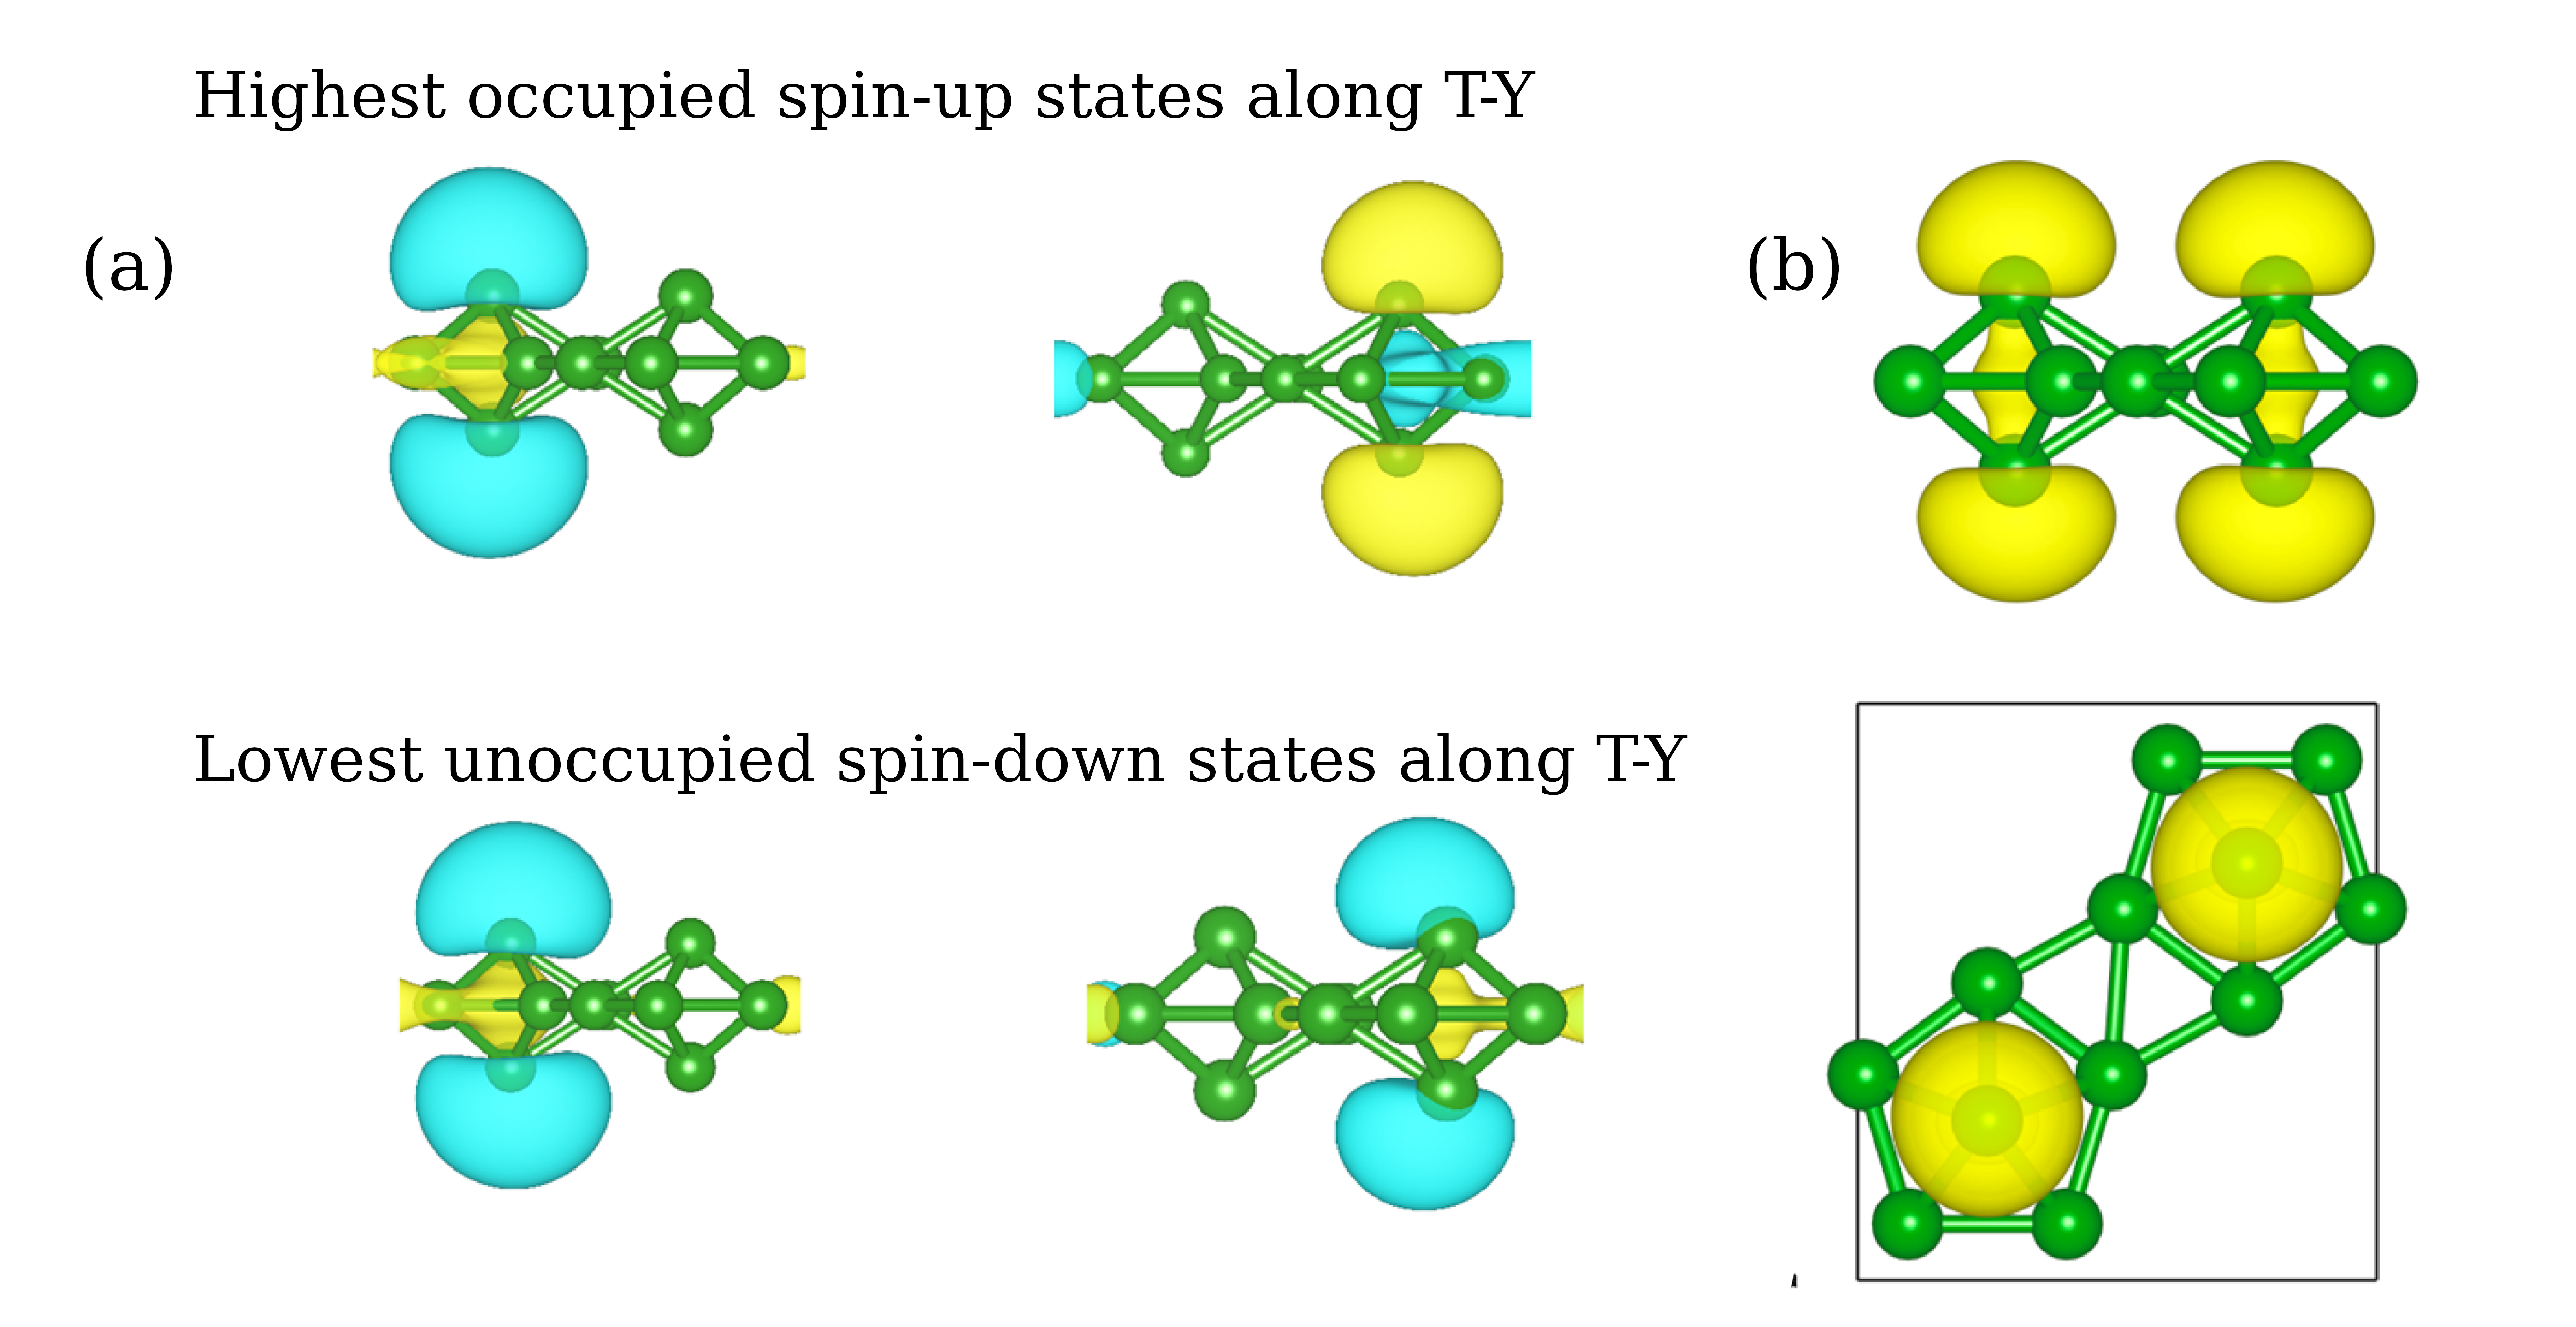
\includegraphics[width=0.75\linewidth]{figures_proj2/S2.17/S2.17.png}
\caption{(a) Highest occupied spin-up state and lowest unoccupied spin-down state of the FM monolayer,
taken midway along the high-symmetry $\mathrm{T}$--$\mathrm{Y}$ direction in the Brillouin zone.
(b) Corresponding spin density,
with an isosurface value of \qty{0.005}{e\per\angstrom\cubed}.}
\label{S2.17}
\end{figure}

\begin{figure}[!htbp]
\centering
    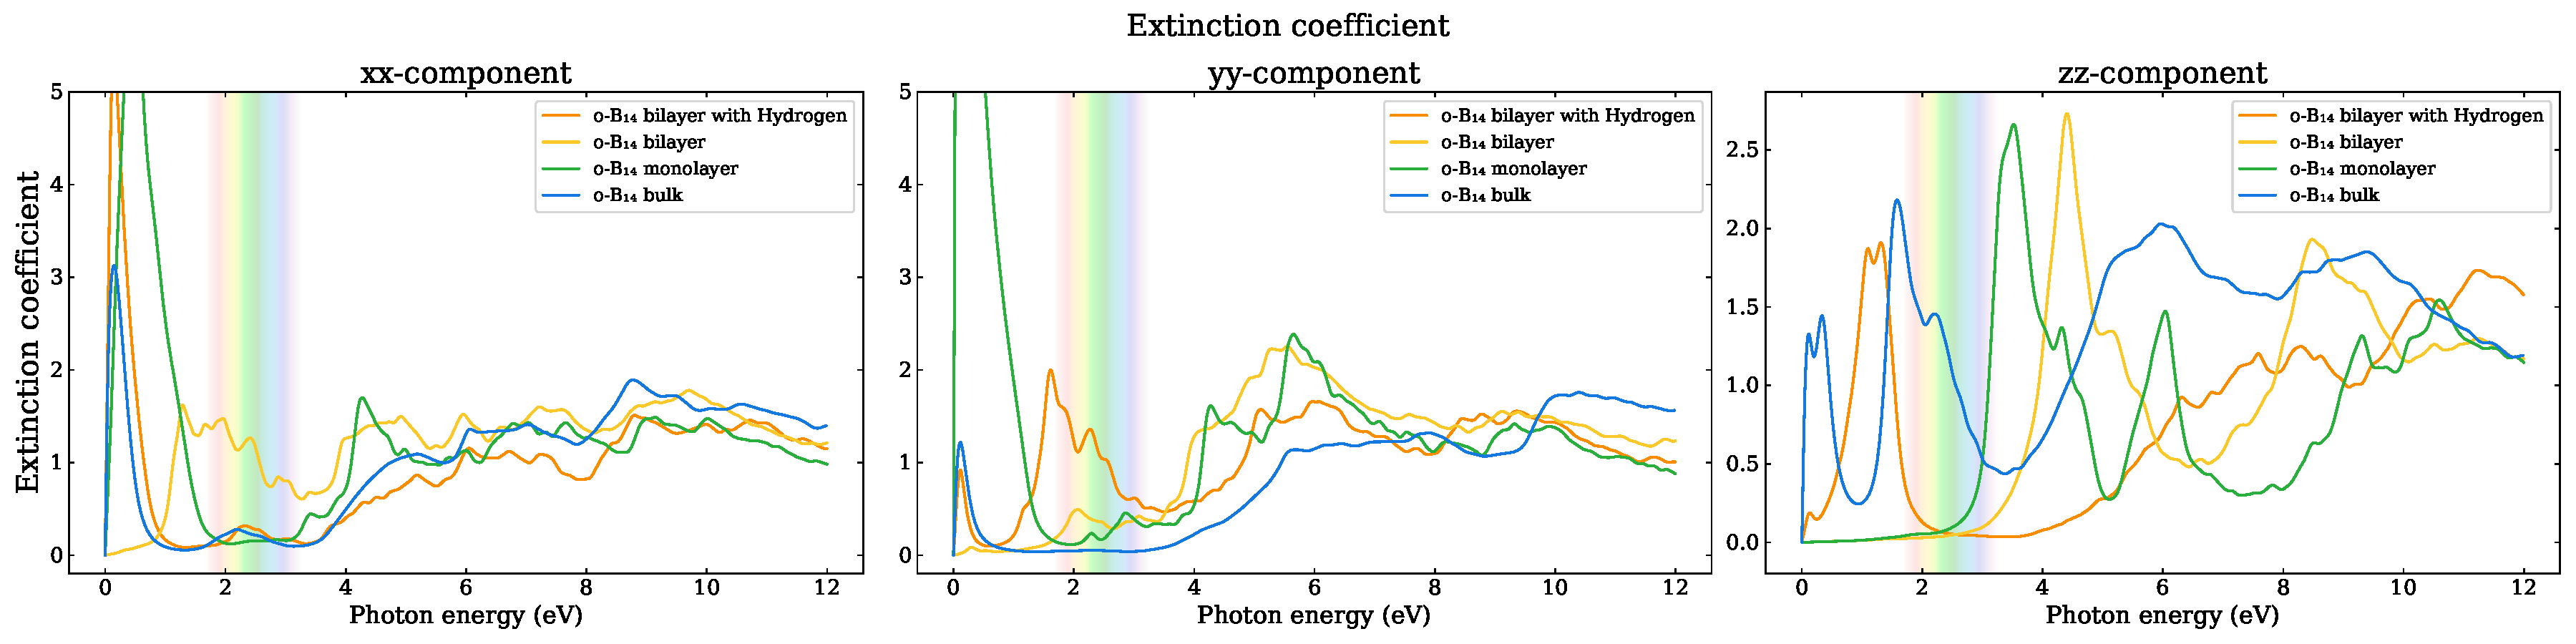
\includegraphics[width=1.0\linewidth]{figures_proj2/S2.18.pdf}
\caption{
Extinction coefficient as a function of energy for the o-\ce{B14} structures along the $xx$, $yy$, and $zz$ directions.
}
\label{S2.18}
\end{figure}
